%% The main file. It contains definitions of basic parameters and includes all other parts.

%% Settings for single-side (simplex) printing
% Margins: left 40mm, right 25mm, top and bottom 25mm
% (but beware, LaTeX adds 1in implicitly)
\documentclass[12pt,a4paper]{report}
\setlength\textwidth{145mm}
\setlength\textheight{247mm}
\setlength\oddsidemargin{15mm}
\setlength\evensidemargin{15mm}
\setlength\topmargin{0mm}
\setlength\headsep{0mm}
\setlength\headheight{0mm}
% \openright makes the following text appear on a right-hand page
\let\openright=\clearpage

%% Settings for two-sided (duplex) printing
% \documentclass[12pt,a4paper,twoside,openright]{report}
% \setlength\textwidth{145mm}
% \setlength\textheight{247mm}
% \setlength\oddsidemargin{14.2mm}
% \setlength\evensidemargin{0mm}
% \setlength\topmargin{0mm}
% \setlength\headsep{0mm}
% \setlength\headheight{0mm}
% \let\openright=\cleardoublepage

\usepackage{import}

\usepackage[usenames]{xcolor}  % typesetting in color
\usepackage{listings}

%% Generate PDF/A-2u
\usepackage[a-2u]{pdfx}

%% Character encoding: usually latin2, cp1250 or utf8:
\usepackage[utf8]{inputenc}

%% Prefer Latin Modern fonts
\usepackage{lmodern}
\usepackage[T1]{fontenc}

\usepackage[toc,page]{appendix}
%% Further useful packages (included in most LaTeX distributions)
\usepackage{amsmath}        % extensions for typesetting of math
\usepackage{amsfonts}       % math fonts
\usepackage{amsthm}         % theorems, definitions, etc.
\usepackage{bbding}         % various symbols (squares, asterisks, scissors, ...)
\usepackage{bm}             % boldface symbols (\bm)
\usepackage{graphicx}       % embedding of pictures
\usepackage{fancyvrb}       % improved verbatim environment
\usepackage{natbib}         % citation style AUTHOR (YEAR), or AUTHOR [NUMBER]
\usepackage[nottoc]{tocbibind} % makes sure that bibliography and the lists
			    % of figures/tables are included in the table
			    % of contents
\usepackage{dcolumn}        % improved alignment of table columns
\usepackage{booktabs}       % improved horizontal lines in tables
\usepackage{paralist}       % improved enumerate and itemize

\usepackage{multirow}

%\usepackage{tkiz}
%\usepackage{pgflibraryarrows}    %Optional
%\usepackage{pgflibrarysnakes}   %Optional
%\usepackage{textcomp}

%% SPECIMEN
% Parts marked as SPECIMEN are used for building the example PDF.
% When the official template is generated by ./mkdist, all such parts
% are deleted, as well as all calls of \X and \XXX macros.
\def\X#1{\textcolor{red}{[#1]}}
\def\XXX#1{\par\smallskip\noindent \textcolor{red}{[#1]}}
%% NEMICEPS

%%% Basic information on the thesis

% Thesis title in English (exactly as in the formal assignment)
\def\ThesisTitle{Thesis title \X{as in the formal assignment}}

% Author of the thesis
\def\ThesisAuthor{Name Surname}

% Year when the thesis is submitted
\def\YearSubmitted{YEAR}

% Name of the department or institute, where the work was officially assigned
% (according to the Organizational Structure of MFF UK in English,
% or a full name of a department outside MFF)
\def\Department{Name of the department \X{as per Organizational Structure of MFF UK in English}}

% Is it a department (katedra), or an institute (ústav)?
\def\DeptType{Department}

% Thesis supervisor: name, surname and titles
\def\Supervisor{Supervisor's Name \X{+titles}}

% Supervisor's department (again according to Organizational structure of MFF)
\def\SupervisorsDepartment{department}

% Study programme and specialization
\def\StudyProgramme{study programme}
\def\StudyBranch{study branch}

% An optional dedication: you can thank whomever you wish (your supervisor,
% consultant, a person who lent the software, etc.)
\def\Dedication{%
Dedication.
}

% Abstract (recommended length around 80-200 words; this is not a copy of your thesis assignment!)
\def\Abstract{%
Abstract. \X{Recommended length around 80--200 words. This is not a~copy of your thesis assignment!}
}

% 3 to 5 keywords (recommended), each enclosed in curly braces
\def\Keywords{%
{key} {words} \X{usually 3 to~5 key words or phrases}
}

\usepackage{hyperref}
%% The hyperref package for clickable links in PDF and also for storing
%% metadata to PDF (including the table of contents).
%% Most settings are pre-set by the pdfx package.
\hypersetup{unicode}
\hypersetup{breaklinks=true}

% Definitions of macros (see description inside)
%%% This file contains definitions of various useful macros and environments %%%
%%% Please add more macros here instead of cluttering other files with them. %%%

%%% Minor tweaks of style

% These macros employ a little dirty trick to convince LaTeX to typeset
% chapter headings sanely, without lots of empty space above them.
% Feel free to ignore.
\makeatletter
\def\@makechapterhead#1{
  {\parindent \z@ \raggedright \normalfont
   \Huge\bfseries \thechapter. #1
   \par\nobreak
   \vskip 20\p@
}}
\def\@makeschapterhead#1{
  {\parindent \z@ \raggedright \normalfont
   \Huge\bfseries #1
   \par\nobreak
   \vskip 20\p@
}}
\makeatother

% This macro defines a chapter, which is not numbered, but is included
% in the table of contents.
\def\chapwithtoc#1{
\chapter*{#1}
\addcontentsline{toc}{chapter}{#1}
}

% Draw black "slugs" whenever a line overflows, so that we can spot it easily.
\overfullrule=1mm

%%% Macros for definitions, theorems, claims, examples, ... (requires amsthm package)

\theoremstyle{plain}
\newtheorem{thm}{Theorem}
\newtheorem{lemma}[thm]{Lemma}
\newtheorem{claim}[thm]{Claim}

\theoremstyle{plain}
\newtheorem{defn}{Definition}

\theoremstyle{remark}
\newtheorem*{cor}{Corollary}
\newtheorem*{rem}{Remark}
\newtheorem*{example}{Example}

%%% An environment for proofs

%%% FIXME %%% \newenvironment{proof}{
%%% FIXME %%%   \par\medskip\noindent
%%% FIXME %%%   \textit{Proof}.
%%% FIXME %%% }{
%%% FIXME %%% \newline
%%% FIXME %%% \rightline{$\square$}  % or \SquareCastShadowBottomRight from bbding package
%%% FIXME %%% }

%%% An environment for typesetting of program code and input/output
%%% of programs. (Requires the fancyvrb package -- fancy verbatim.)

\DefineVerbatimEnvironment{code}{Verbatim}{fontsize=\small, frame=single}

%%% The field of all real and natural numbers
\newcommand{\R}{\mathbb{R}}
\newcommand{\N}{\mathbb{N}}

%%% Useful operators for statistics and probability
\DeclareMathOperator{\pr}{\textsf{P}}
\DeclareMathOperator{\E}{\textsf{E}\,}
\DeclareMathOperator{\var}{\textrm{var}}
\DeclareMathOperator{\sd}{\textrm{sd}}

%%% Transposition of a vector/matrix
\newcommand{\T}[1]{#1^\top}

%%% Various math goodies
\newcommand{\goto}{\rightarrow}
\newcommand{\gotop}{\stackrel{P}{\longrightarrow}}
\newcommand{\maon}[1]{o(n^{#1})}
\newcommand{\abs}[1]{\left|{#1}\right|}
\newcommand{\dint}{\int_0^\tau\!\!\int_0^\tau}
\newcommand{\isqr}[1]{\frac{1}{\sqrt{#1}}}

%%% Various table goodies
\newcommand{\pulrad}[1]{\raisebox{1.5ex}[0pt]{#1}}
\newcommand{\mc}[1]{\multicolumn{1}{c}{#1}}


%%% MY MACROS
\newcommand{\todoA}[1]{[TODO A: #1]}  % urcite nutno
\newcommand{\todoB}[1]{[TODO B: #1]}  % bylo skoda to tam nedat
\newcommand{\todoC}[1]{[TODO C: #1]}  % pridal bych kdybych mel cas

\newcommand{\jh}[1]{[JH: #1]}  % komentar Jiriho Hany


% Title page and various mandatory informational pages
\begin{document}
%%% Title page of the thesis and other mandatory pages

%%% SPECIMEN
%%% Inscriptions at the opening page of the hard cover
\todoA{remove}

\pagestyle{empty}
\hypersetup{pageanchor=false}
%\XXX{Opening page of the hard cover. Not a part of the electronic version.}
\begin{center}

\large
Charles University

\medskip

Faculty of Mathematics and Physics

\vfill

{\huge\bf BACHELOR THESIS}

\vfill

\hbox to \hsize{\YearSubmitted\hfil \ThesisAuthor}

\end{center}

\newpage\openright

%%% NEMICEPS

%%% Title page of the thesis

\pagestyle{empty}
\hypersetup{pageanchor=false}
\begin{center}

\centerline{\mbox{
\includegraphics[width=166mm]{../img/logo-en.pdf}}}

\vspace{-8mm}
\vfill

{\bf\Large BACHELOR THESIS}

\vfill

{\LARGE\ThesisAuthor}

\vspace{15mm}

{\LARGE\bfseries\ThesisTitle}

\vfill

\Department

\vfill

\begin{tabular}{rl}

Supervisor of the bachelor thesis: & \Supervisor \\
\noalign{\vspace{2mm}}
Study programme: & \StudyProgramme \\
\noalign{\vspace{2mm}}
Study branch: & \StudyBranch \\
\end{tabular}

\vfill

% Zde doplňte rok
Prague \YearSubmitted

\end{center}

\newpage

%%% Here should be a bound sheet included -- a signed copy of the "bachelor
%%% thesis assignment". This assignment is NOT a part of the electronic
%%% version of the thesis. DO NOT SCAN.
\XXX{Bound into the introductory part must be the form with signed approval of the thesis topic (a photocopy suffices).
This is not a~part of the electronic version of the thesis, do not scan!}

%%% A page with a solemn declaration to the bachelor thesis

\openright
\hypersetup{pageanchor=true}
\pagestyle{plain}
\pagenumbering{roman}
\vglue 0pt plus 1fill

\noindent
I declare that I carried out this bachelor thesis independently, and only with the cited
sources, literature and other professional sources.

\medskip\noindent
I understand that my work relates to the rights and obligations under the Act No.~121/2000 Sb.,
the Copyright Act, as amended, in particular the fact that the Charles
University has the right to conclude a license agreement on the use of this
work as a school work pursuant to Section 60 subsection 1 of the Copyright Act.

\vspace{10mm}

\hbox{\hbox to 0.5\hsize{%
In ........ date ............	% FIXME!
\hss}\hbox to 0.5\hsize{%
signature of the author
\hss}}

\vspace{20mm}
\newpage

%%% Dedication

\openright

\noindent
\Dedication

\newpage

%%% Mandatory information page of the thesis

\openright

\vbox to 0.5\vsize{
\setlength\parindent{0mm}
\setlength\parskip{5mm}

Title:
\ThesisTitle

Author:
\ThesisAuthor

\DeptType:
\Department

Supervisor:
\Supervisor, \SupervisorsDepartment

Abstract:
\Abstract

Keywords:
\Keywords

\vss}

\newpage

\openright
\pagestyle{plain}
\pagenumbering{arabic}
\setcounter{page}{1}


%%% A page with automatically generated table of contents of the bachelor thesis

\tableofcontents

%%% Each chapter is kept in a separate file
\chapter*{Introduction}
\addcontentsline{toc}{chapter}{Introduction}

%Charming decore. Delicious food. Friendly staff. We'll certainly become repeat customers.", "useful": 2


With growing popularity of storing and sharing more data on the internet, the biggest challenge
for us is not to get enough information, but to find the exact information we need.
This thesis aims to tackle one of the major issues of review systems.
A review system is a platform for sharing experience among its users.
It is particularly aimed at information that is hard to find in another way than from direct experience.
The information is often subjective and relevant only in a narrow context.
A review of a novel praising historical accuracy may be interesting to a history teacher,
but not so much to someone who only searches for a gripping story.

In particular, users use review systems for obtaining some information based on the experience of others.
The users are often willing to spend only a couple of minutes on finding relevant information to them.
Usually, the review systems contain many reviews and review systems tries to improve the user experience by showing useful reviews first.

We work with reviews of restaurants from the online platform Yelp.
It works in a similar manner like other recommendation systems such as IMDB\footnote{Internet Movie Database \url{https://www.imdb.com/}} or
TripAdvisor.\footnote{\url{https://www.tripadvisor.com}}
There are restaurant profiles to which users can add reviews based on their recent visit.
An example of a profile is shown in \Cref{fig:dobra_trafika}.

\begin{figure}[ht]\centering
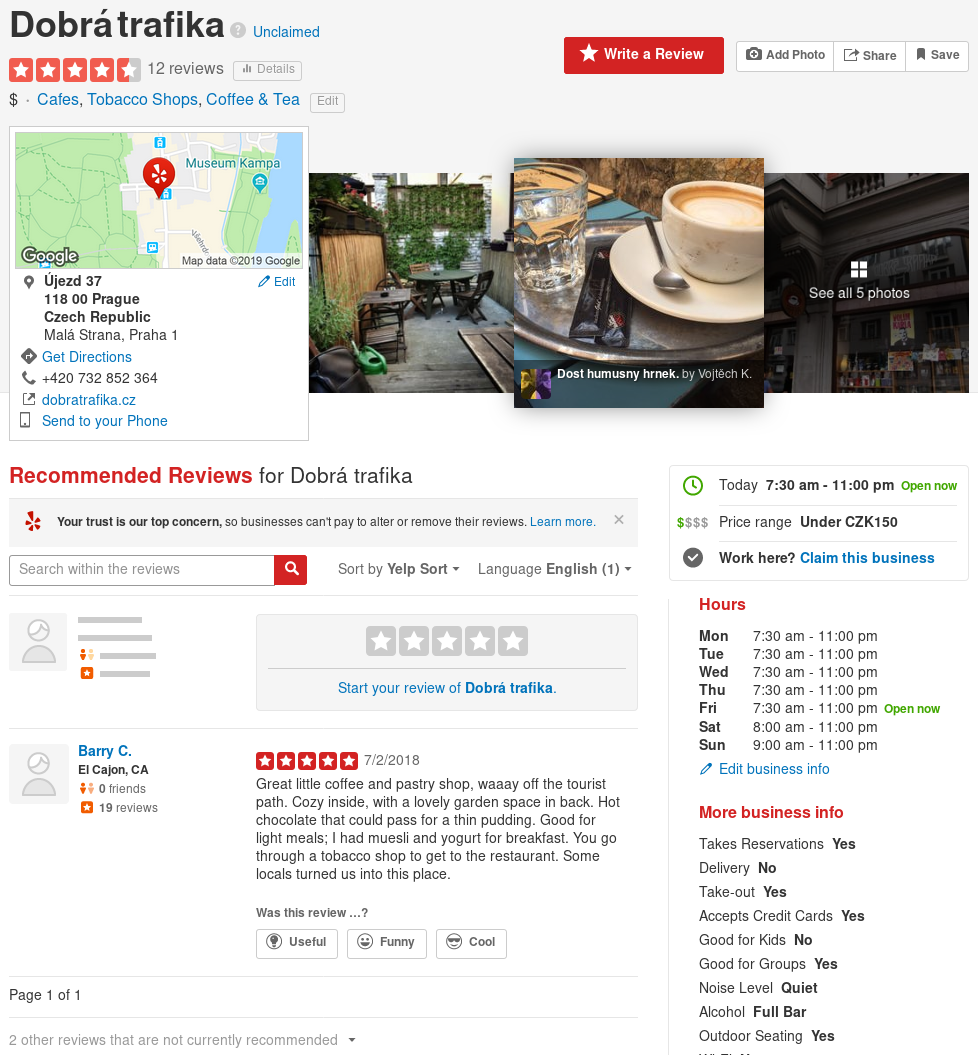
\includegraphics[width=130mm]{../img/dobra_trafika.png}
\caption{An example of an online profile}
\label{fig:dobra_trafika}
\end{figure}

A typical review of a restaurant looks like this:

\begin{code}
Charming decore. Delicious food. Friendly staff.
We'll certainly become repeat customers.
\end{code}

It contains unformatted pieces of information, fragments of sentences or typos.
In general, it can contain anything and \citet{Song14} define it as a new genre --- \textbf{short text}.
Short text is used in e-commerce systems and online communication in general.
It is usually up to 200 characters per document.
It is characterizes by its sparsity, free form and being large-scale and in the real time.
Although an average review in our data has 526 characters, we consider this short text.
First, it fulfills other characteristics.
Second, the bounds are not clearly defined.
An example of another short text system is Instant Messaging software Windows Live Messenger allowing up to 400 characters.

The reasons listed above make it difficult to work with short text.
Furthermore, there are many factors contributing to the difficulty of finding useful reviews.
First, we do not know the author and possibly have only a few reviews by the author.
Also, reviews by the same author can have different quality which is influenced by many factors,
such as the time spent on writing the review or whether the actual experience contains some useful information.
Therefore it is very hard to estimate author's reliability.
Second, reviews are very short, often containing only one piece of information.
Third, a review can quickly become obsolete or irrelevant.
Fourth, what is relevant to some, may not be to others.
All this also makes the task hard even for human operators and as such hard to evaluate our programme selecting useful reviews.

The main reason we chose Yelp is that users can flag properties of other reviews in the form of \emph{likes}.
Each review has three buttons --- \emph{useful}, \emph{funny} and \emph{cool} as can be seen in \Cref{fig:dobra_trafika}.
A user can vote for the property of a review by clicking on one of these buttons.
A typical review flagged as useful looks like this:

\begin{code}
A proper greasy spoon.
I was looking for a bacon flavoured hangover cure and I got one.
And a proper builders mug of tea.
Cheap as chips as well.
\end{code}

It clearly mentions the kind of the restaurant, what to seek there,
who it can be for and price.

On the other hand, a typical not-useful review looks like this:

\begin{code}
Awesome keg.. Always good, even with my own money!
\end{code}

It does only mention the place is good, but does not explain why --- price, friendly staff, location\dots.
The mention about money is unclear.
Does it mean the author has not got much money and therefore appreciate their cheap prices? Or something else?

Sometimes the review is not of a big quality itself, but contains some piece of information which makes it useful.
The review bellow is of a poor quality, not well formatted and only mentioning that we should not go there.
However, the mention about the bouncer and the tip turns out to be very useful for many users,
because it informs about the additional expenses added to the cost.

\begin{code}
Dont bother...this place is a dive!
The bouncer demanded a tip, just to seat us...def seek elsewhere...
you've been warned!!!
\end{code}

Of course, it is often near to impossible to decide whether a review is useful or not.
The review bellow clearly expresses pros and cons.
It is not a place to go when in hurry, not great for some delicious food,
but it is alright when we are not in hurry and want to have a friendly service.
However, the points are somewhat vague and the review is very subjective.

\begin{code}
It was OK. Service was friendly, but slow.
Food was OK, but I don't think it was a good value.
\end{code}


More about the data and the platform can be found in \Cref{app:dataset}.

Our objective is to create a software package that predicts whether some users would flag a restaurant review as a useful.
This prediction can be used for filtering out only useful reviews in a real review system.
We utilize means of supervised binary classification.
The useful likes are used for labelling reviews as \textit{useful} and \textit{not-useful}.
To ensure they have been viewed by enough users to get enough likes,
we take reviews only from a particular time frame
and we use only frequent restaurants with detailed profiles for the same reason.
We focus on classification of English reviews.

This is a well studied field and to date, many approaches to solve this have been introduced.
However, there is no clearly best performing algorithm for particular application.
Our main goal is therefore to compare already existing approaches.
The results can serve as a guide when implementing a real review system.

\section{Roadmap}

In \textbf{\Cref{chap:cls} Text Classification}, we define our task properly as text classification and briefly mention classification in different contexts.
We describe the utilized machine learning methods with examples of concrete usage.

In \textbf{\Cref{chap:fea} Feature Engineering}, we discuss several possibilities how to extract properties called features from text and how to filter only those useful.
Next, we mention dimension reduction as a possibility to reduce the complexity of our solution.
Finally, we introduce several commonly used features and filtering methods.
To a lessen degree, we also talk about non-textual data as well.

In \textbf{\Cref{chap:eval} Evaluation}, we introduce methods for comparing different algorithms.
We describe what requirements we expect a good algorithm to satisfy and how to use the data for comparing performance.
Lastly, we mention commonly used metrics to give us some easily comparable numbers.

In \textbf{\Cref{chap:arch} The Software Project Architecture}, we describe at the conceptual level our software package.
We describe individual modules, how they interact and the overall project structure.
We also talk about different files and configuration the project needs and commands used for running the project.

In \textbf{\Cref{chap:exp} Conducted Experiments}, we outline the experiments.
We describe combinations of algorithms we used and discuss the results.
We justify the compromises made for performance reasons.
Finally, we talk about the impact of size of the data to the performance.

In \textbf{\Cref{app:dataset} Yelp Dataset},
we describe the source of the data and its exact format.
We demonstrate how reviewing of businesses work and
the exact format of the data.

In \textbf{\Cref{app:prepr} Data Preprocessing},
we describe the challenge of obtaining reliable data and
what preprocessing has been done to allow easier manipulation and increase in reliability of the usefulness metrics.

In \textbf{\Cref{app:geneea} Geneea Data},
we describe the NLP analysis used for extracting sentiment and entities.

In \textbf{\Cref{app:techn} Package Technicalities},
we describe technical details and peculiarities of the software package.
We also provide commands for running the experiments and specify configuration.

In \textbf{\Cref{app:mi} Top Features by Mutual Information},
we list mutual information of selected features.


\section{Typographic Conventions}

In this thesis, we use the following typographic conventions:

\begin{itemize}
\item \textbf{bold} for definitions of new terms

\item \textit{italics} for mentions of already defined names. It also denotes data files in \Cref{chap:arch}.

\item \texttt{monospace} is used for code and filenames. It is used for process names in \Cref{chap:arch}.

\end{itemize}

\section{Related Work}

A lot of research has been done in short text classification.
Executive summary can be found in \citet{Song14}.
They define short text as a new genre; listing its characteristics, summarizing possible approaches to short text classification and evaluating performance.

One of the well studied dataset is tweets from Twitter.\footnote{\url{https://twitter.com}}
A lot of studies on sentiment analysis have been conducted.
\citet{jiang2011target} allege that most approaches follow
\citet{pang2002thumbs} who utilize machine learning based classifiers;
the state-of-the-art being \citet{go2009twitter} and \citet{barbosa2010robust}.
Perhaps more relevant study on Twitter is \citep{sriram2010short},
which tackles the problem of filtering relevant information.

Reviews are to author's knowledge less studied.
One of the relevant papers is \citet{ganu2009beyond}.
They discuss the difficulties of selecting useful restaurant reviews.
Unlike this thesis, they do not classify reviews as a whole, but instead try to find reviews containing topics such as food or service.
The main attempt is to find some structure in the free form.

Related text classification research focuses on sentiment analysis and toxic speech detection.
A lot of research is focusing on sentiment analysis.

Relatively close research focuses on toxic speech.
\citet{van2018challenges} talk about toxic speech as non-constructive and non-inclusive conversation including hate speech, threats, insults and in general fruitless conversation.
Filtering out fruitless text is our focus to high extent too.
Apart from already mentioned challenges they mention high variance in performance and difficulty to define the topic clearly.
Basic review of toxic speech classification can be found in \citet{gunasekara2018review}.

\chapter{Yelp Open Dataset}

Yelp is a US-based company whose goal is: ``to connect people with great local businesses.''\footnote{\url{https://yelp.com/about}}
It provides both mobile and web interface listing businesses such as restaurants or shopping centres.
Users can easily post a review for any business based on their recent visit.
All this makes the platform very popular and because of its convenience many people review businesses.

There are three main reasons we chose to evaluate our algorithms on this dataset.
As we mentioned this platform is very popular and as such has sufficient data.

Secondly, the company publishes every year an open dataset which can be downloaded for academic
purposes.
It covers most information conveyed in their system ---  information about businesses and users, pictures taken by the users and most importantly for us textual reviews.
As such it is possible to download the entire dataset without having to scrape some data.

Lastly, this dataset allows us to asses the needed properties of individual reviews.
The platform not only allows users to post reviews, but also to asses other reviews in form of \emph{likes}.
Each review has three buttons --- \emph{useful}, \emph{funny} and \emph{cool}.
A user can express the property of a review by clicking on one of these buttons. Information how many times these buttons have been clicked is also present in the dataset and as such makes it a great dataset for evaluating how well our algorithms perform.

\todoA{very brief mention about dataset format and link to appendix}

\chapter{Text Classification}

% \begin{tikzpicture}
%   \begin{scope}[blend group = soft light]
%     \fill[red!30!white]   ( 90:1.2) circle (2);
%     \fill[green!30!white] (210:1.2) circle (2);
%     \fill[blue!30!white]  (330:1.2) circle (2);
%   \end{scope}
%   \node at ( 90:2)    {Typography};
%   \node at ( 210:2)   {Design};
%   \node at ( 330:2)   {Coding};
%   \node [font=\Large] {\LaTeX};
% \end{tikzpicture}

The process of~selecting useful review is an example of {\bf text classification}.
\citet{AggZhai12} describe text classification as follows.
We have records~$X_1, \ldots, X_N$ and labels~$1,\ldots, k$.
Record is a standalone unit and is assigned one label.
Text classification aims to predict what label it is.

Every record consists of~attributes which convey some~information about it.
An example of an attribute is the text of a review or the number of stars given by the user.
We will refer to a~record as {\bf an~instance} to be consistent with machine learning terminology.
{\bf Text classification} is then a process of building a classification model that is able to assign
an instance its label based solely on its attributes.
{\bf Classification model} (also called classifier) is a~mapping between an~instance and a~class label.

\todoA{diagram records -> labels - records=instances; labels; arrows are the model}
	\begin{code}
		review            -->        useful

		review2		-->			not-useful


		review3 arrow up

		^^^^^^^						^^^^^
		instance					labels

		arrows = model
	\end{code}


As \citet{TanBachKum08} distinguish it, classification is either {\it descriptive} and {\it predictive}.
Descriptive is for finding regularities in data.
An example of descriptive classification is a task where
biologists try to figure out what the features distinguishing mammals and birds are.
In this thesis, we will consider only predictive classification, where the goal is to build a classifier
that can predict labels for new instances.

We have two sets of instances to be able to asses how well our model predicts instances.
First, a training set is  used for building a~classification model.
Second, a testing set is used for assessing how well the model predicts labels for new instances.
Because the testing set contains the actual labels, we can compare our predictions with them.

The approach of fitting a classifier to labelled data is called \textbf{supervised learning}.
We have the results of classification and we are trying to build a model that approximates these results.
On the contrary, \textbf{unsupervised learning} means that we do not know the labels and we try to group instances that are in some respect similar without having labels.

In~this thesis, we take into account only \textbf{hard version} of~classification which explicitly maps one and only one label to each record.  
\textbf{Soft version} assign probabilities to labels.

\section{Text Classification Process}

TODO - tady jsme skoncili - prepsat tohle neni hezke

The process of classification is broken down into four parts as shown in \autoref{fig:cls_process}.

\todoA{diagram:}
\begin{figure}
\begin{code}
obtaining dataset
-> preprocessing {extraction} -> feature selection
 ^^^^^^^^^^^^^^^^^^^^^^^^^^^^^^^^^^^^^^^^^^^^^^^^^^^^^^
    		feature engineering

-> training -> evaluation
\end{code}
	blah\label{fig:cls_process}
\end{figure}


We always need to obtain sufficient information about each instance.
This mean we can use more sources.
Obtaining data usually comprises of data scraping or otherwise downloading it.
We do not cover this, because the Yelp dataset is freely available for download.

We cannot feed the data directly into our classifier.
The data has to be preprocessed first.
This process is called {\bf feature engineering}.
We extract the so called {\bf features}, which carry some information about the instance.
Feature is simply some property of an instance like the number of words in a review.
As we will see, it is hard to come up with features that would directly lead to successful classification.
Hence, we will try to generate as many features as we can and then try to select the most useful.
We will discuss both feature extraction and selection in \autoref{chap:fea}.


Once the data is ready, we build a classifier from the preprocessed data.
This phase is called training.
Finally, we want to be able to compare different classifiers and feature sets.
Common evaluations will be discussed in \autoref{chap:eval}.

Last three chapters  are left for the architecture of the software developed (\autoref{chap:arch}),
demonstration of conducted experiments (\autoref{chap:exp}) and final discussion (\autoref{chap:concl}).



\section{\todoB{What a Classifier Looks Like}}

\todoB{Probabilistic model for classification
Generally speaking, there are two models used for classification; generative and discriminative. Generative model assumes there exist }

\subsection{\todoB{hyperparameteres, parameters, model}}

\subsection{\todoC{discrm. vs generative}}

\todoB{linear classifier def}

\section{Classifiers}
\label{chap:clscon}

As we mentioned, classification is a process of building a classification model which maps
instances onto labels.
In this section, we will describe some commonly used classifiers.
We will demonstrate them on mock data shown in \autoref{tab:custsatis}.
We have a fictional dataset of customers of a mobile carrier and
we are trying to predict whether customers are satisfied.
The rows are instances and columns features.
Our three features are 
whether the customer received a discount (yes or no), whether it is a private customer (yes or no)
and what mobile internet is part of their prepaid plan (none, limited and unlimited).
We are predicting the last column.

Please note that our primar focus is text classification.
However, we will use non-textual features in this example for easier understanding.
Classifiers (except for fastText which is tailored specifically for text) take any set of features,
so we can use them in the same way with features extracted directly from text.
We will learn how to do that in \autoref{chap:fea}.

\begin{table}[h!]

\centering
\begin{tabular}{lllll}
\toprule
\textbf{ID} & \textbf{discount} & \textbf{private} & \textbf{internet} \hspace{1.cm} & \textbf{satisfied} \\
\midrule
1 & yes & yes & unlimited & yes \\
2 & no & yes & unlimited & yes \\
3 & no & no & unlimited & no \\
4 & yes & yes & no & yes \\
5 & no & yes & limited & no \\
6 & yes & no & limited & yes \\
7 & no & yes & no & no \\
\bottomrule
\end{tabular}

\caption{Customer satisfaction example}\label{tab:custsatis}
\end{table}






\subsection{Zero-R, One-R}

These two algorithms are used as a baseline.
Baseline algorithm is a very simple method used to get better idea about the dataset and dificulty of our task.
It is useful to have a comparison to whatever more sophisticated we developed.
Suppose, we have a very sophisticated classifier predicting 22\% instances correctly
We may lean to say that the performance is not really good.
And if the baseline gets 20\% well, it may really be that case.
However, when our baseline predicts only 3\%, 22\% may be actually very good results worth the effort.

{\bf Zero-R} simply takes the most frequent label and labels every instance with it.
Zero-R would label all customers as satisfied in our example.

A bit more complicated {\bf One-R} chooses one feature and bases the classification solely on this feature.
For every value of the feature, we take all instances corresponding to this value and choose the label occurring the most among them.
For predicting, we use the label we found for each value.

Suppose we choose the feature {\it discount} in our example.
We can see that all customers that got discount are satisfied.
Hence all customers getting a discount are according to one-R satisfied.
Three customers that did not get discount are dissatisfied and one is satisfied.
Hence one-R will predict all customers without a discount as dissatisfied.

The problem is how to choose the most informative feature which we will tackle in \autoref{subsec:decisiontree}.
For now we can think of it as finding such a feature, that will produce the best classifier.

\subsection{Na\"{i}ve Bayes}

Na\"{i}ve Bayes is a probabilistic classifier.
Probabilistic means that we classify an instance according to the probabilities of the instance belonging to individual classes (having that label).
Mathematically speaking, we choose label~$\hat{c}$~from the set of all labels $C=\left\{c_1,c_2,\dots c_n\right\}$ for instance~$d_j$, such that:

\begin{equation}
	\label{eq:argmax}
	\hat{c} = \argmax_{c_i \in C} P\left(c_i  | d_j \right),
\end{equation}

where~$P\left(c_i | d_j\right)$~is the probability of~$d_j$~being labelled with~$c_i$.
Note that we use \textit{arg\,max} which equals to the value of the argument variable
with the highest value of the expression.

However, we do not directly say what label belongs to the instance we are predicting.
Instead, Na\"{i}ve Bayes uses the so-called generative model.
In generative model, we assume every instance is generated by a parametric model.
\textbf{Parametric model} consists of~$n$~components $c_1, c_2,\ldots, c_n$.
Every component corresponds to one class label
and is said to generate all instances with this label.
Note that since there is one-to-one correspondence between classes and components,
we use the same notation for both components and labels.
It should be clear from the context what we mean (i.e. component generates an instance,
but an instance is assigned a label).
Also note, that the assumption about class and component correspondence is only used for simplification and can be generalised \todoA{source}.

An instance is generated in two steps.
First, a component is selected according to priors.
Priors are the apriori probabilities of the current model denoted by $P\left(c_i\right)$ for component~$c_i$.
Second, an instance is generated by this component according to posterios.
Posteriors are probabilities of instance~$d_j$~being generated by component~$c_i$~denoted by~$P\left(d_j|c_i\right)$.

The likelihood of instance~$d_i$~being generated is then:

\begin{equation}
	P\left(d_j\right) = \sum_{i=1}^{n}{
	P\left(c_i\right)
	P\left(d_j|c_i\right)
}
\end{equation}

Next, we need to convert these probabilities into the probability of an instance having a label.
We can infer \autoref{eq:bayesrule} (called \textbf{Bayes rule}) from \autoref{eq:bayesinfer}.

\begin{equation}
	\label{eq:bayesinfer}
	P\left(A,B\right) = 
	P\left(A|B\right)
	P\left(B\right) = 
	P\left(A\right)
	P\left(B|A\right),
\end{equation}
\begin{equation}
	\label{eq:bayesrule}
	P\left(A|B\right) =
	\frac{
	P\left(A\right)
P\left(B|A\right)}
{P\left(B\right)}
\end{equation}

Our original \autoref{eq:argmax}

\begin{equation}
	\hat{c} = \argmax_{c_i \in C} P\left(c_i  | d_j \right)
\end{equation}

can be transcribed with Bayes rule as:

\begin{equation}
	\hat{c} = \argmax_{c_i \in C}
	\frac{
	P\left(d_j  | c_i \right)
	P\left( c_i \right)
}{
	P\left( d_j \right)
}
\end{equation}

Because we are not interested in the exact value of the expression, it is equivalent to:

\begin{equation}
	\label{eq:classprb}
	\hat{c} = \argmax_{c_i \in C}
	P\left(d_j  | c_i \right)
	P\left( c_i \right)
\end{equation}

The exact values of probabilities are calculated as follows.
Prior probabilities are the distribution of classes.
The exact values are computed by counts.
For computing posterios, Na\"{i}ve Bayes assumption is used.
It says that each feature is independent of all other features.
Note that in practical context, the assumption often does not hold.
However, since we are only interested in the label with highest probability,
not the probability itself, possible errors are often insignificant and Na\"{i}ve Bayes often works in practise even when the features are not independent.
Thanks to the assumption, the probability of an instance represented by feature values is the product
of probabilities of individual features having the given values.
For features $f_1, f_2, \dots f_K$ it is:

\begin{equation}
	\label{eq:posterios}
	P\left(d_j  | c_i \right) = \prod_{k=1}^{K}
	{P\left(  f_k  | c_i \right)}
\end{equation}

By combining \autoref{eq:classprb} and \autoref{eq:posterios}, we get:

\begin{equation}
	\hat{c} = \argmax_{c_i \in C}
	\prod_{k=1}^{K}
	{P\left(  f_k  | c_i \right)}
	P\left( c_i \right)
\end{equation}

Probability~$P\left(f_k|c_i\right)$~is found by counting.
We take all instances from class~$c_i$~and the probability is the ratio of all those instances with the same value of feature~$f_k$~and the rest.

Let us classify instance~$\mathit{ID}=2$~from our mock data in \autoref{tab:custsatis} for demonstration.
For label ``yes'' (satisfied customers):

\begin{equation}
	t_{yes} = 
	\prod_{k=1}^{K}
	{P\left(  f_k  | c_{yes} \right)}
	P\left( c_{yes} \right)
\end{equation}

\begin{equation}
	t_{yes} = 
	P\left(  f_{dis} = no | c_{yes} \right)
	P\left(  f_{priv} = yes | c_{yes} \right)
	P\left(  f_{int} = unlim | c_{yes} \right)
	P\left( c_{yes} \right)
\end{equation}

$P\left(  f_{dis} = no | c_{yes} \right)$ equals $\frac{1}{4}$, because there are four satisfied customers
and only one of them did not receive discount.
Analogously, the remaining values are computed.
$P\left( c_{yes} \right)$ is $\frac{4}{7}$, because there are four satisfied customers out of seven.
Together we get:

\begin{equation}
	t_{yes} = 
	\frac{1}{4} \times
	\frac{3}{4} \times
	\frac{2}{4} \times
	\frac{4}{7}
	\sim 0.054
\end{equation}

We compute~$t_{no}$~in the same manner for a dissatisfied customer:

\begin{equation}
	t_{no} = 
	\prod_{k=1}^{K}
	{P\left(  f_k  | c_{no} \right)}
	P\left( c_{no} \right)
\end{equation}

\begin{equation}
	t_{no} = 
	P\left(  f_{dis} = no | c_{no} \right)
	P\left(  f_{priv} = no | c_{no} \right)
	P\left(  f_{int} = unlim | c_{no} \right)
	P\left( c_{no} \right)
\end{equation}

\begin{equation}
	t_{no} = 
	\frac{3}{3} \times
	\frac{2}{3} \times
	\frac{1}{3} \times
	\frac{3}{7}
	\sim 0.095
\end{equation}

$t_{no}$ is higher and Na\"{i}ve Bayes classifies the instance as dissatisfied.
Note that this may look surprising as features ``private'' and ``internet'' suggest satisfaction,
but the correlation between discount and satisfaction is so strong that it outweights other features in this settings.

\todoC{zminka prior a posterior ohledne maximizace je prave pocitani}



\subsection{Decision trees}
\label{subsec:decisiontree}
\todoC{Decision trees - if you decide not to do it, change ONE-R reference to evaluation}

\subsection{FastText}

FastText\footnote{\url{https://fasttext.cc}} is a small library developed by Facebook.
Text classification in this library is on par with current state-of-the-art deep learning classifiers
and many orders of magnitude faster~\citep{Joulin2017bag}.

Let us first explain a baseline algorithm on top of which fastText builds.
It uses {\it bag of words}\footnote{more on this in the subsection~\ref{subsec:bow}} as features.
This means that each instance is represented by a vector of numbers.
Every position in the vector corresponds to a particular word in a dictionary.
The value of the position denotes number of occurrences of the words in the instance.
A linear classifiers is trained on this.
Linear in this context means that the decision on classification is based on a linear combination of features.
Thanks to this, linear models are a lot faster than complicated neural networks, however the classification may not be as good.

FastText uses {\it word embeddings}\footnote{see the subsection~\ref{subsec:wordembed}} instead of a simple bag of words.
In short, it maps every word onto a vector. Every document is represented as an average vector of all words.

However, fastText goes even further.
The process is precisely described in \citet{Bojanowski2017enriching}.
we will only briefly summarize it.
Fasttext maps n-grams onto vectors, not words.
{\bf N-gram} is any sequence of n elements --- in this case letters.
The algorithm represents a words as an average of vectors of all its n-grams.
Let~$w_{a}$~be a vector representation of an n-gram~$a$, then 
the representation of \texttt{where} is the average of vectors
$w_{whe}$, 
$w_{her}$ and
$w_{ere}$.

For even higher performance, every word is surrounded by \texttt{<} and \texttt{>}.
The word \textit{ where} thus becomes \texttt{<where>}.
The vector of \texttt{where} becomes the average of vectors
$w_{<wh}$, 
$w_{whe}$, 
$w_{her}$,
$w_{ere}$ and
$w_{er>}$.
Note that trigram {\tt her} from \texttt{<where>} is different from {\tt <her} from the word {\tt <here>}.
It allows even better performance, because it distinguishes n-grams at the word boundaries and in the middle.

This approach has a few advantages.
Even words that are not seen during the training phase can be given a vector.
This is especially useful for languages with large vocabularies and many rare words.
Also, unlike the baseline approach, it covers the internal structure of words.
It is useful for morphologically rich languages such as Finnish or Turkish.
Finish has 15 different cases for nouns.
Many of which may not appear in the training set at all.
Hence being able to reasonably represent even unseen words is a big advantage,
because many words follow word formation rules which can be captured in n-grams.
Other implementations represent unseen words with some kind of dummy vector.

As we mentioned, every instance is average of vectors of its words.
This representation is used for training a simple linear classifier.
FastText uses some more tricks to reduce memory consumption and performance.
More details can be found in~\citet{Joulin2017bag}.

\todoA{a budeme muset pridat linearni model - pridej zminku o tom, jak se to klasifikuje podle toho, jestli nekde popises linearni modely vice}

\todoC{hierarchichal softmax}

\subsubsection{\todoC{GloVe - GloVe nepouzivam}}

\subsection{\todoC{NN}}

\subsection{\todoC{Let you imagination go wild}}


\section{\todoB{interpretability -see w8}}

\chapter{Feature Engineering} \label{chap:fea}

In this chapter, we talk about creating features used by the algorithms
introduced in the previous chapter.
We create features and discuss how to find those that are the most informative.
Finally, we describe concrete features we used for the classification.

We cannot use the raw data for training as it is.
Instead, we represent each instance by a set of features;
each feature expressing a certain property of the instance.
An example of a feature can be the number of words in the review,
whether the~word {\it food} is present in the review
or a piece of metadata, like how many stars the user gave.

Features are of three types according to their values~---~nominal, ordinal and continuous.
Nominal features are discrete and there is no relationship between their values.
When a~feature is ordinal, it means it is discrete and also defines an ordering of the values.
Continuous feature is any real-valued variable.

In this thesis, we utilize nominal and ordinal only.
For easier manipulation,
we omit the order in ordinal features and work with them the same way as nominal.
This of course loses information conveyed in this ordering,
but allows us easier feature manipulation.

Feature engineering is a crucial part of the classification process,
because even the best classifiers are helpless without good features.
\citet{liu2012feature} even claim it is likely the most important part.
For this reason, a lot of attention has been dragged towards choosing the right features
and several techniques for doing so were introduced.



\section{Extraction}

\textbf{Feature extraction} is the process of computing feature values for individual instances.
This may involve various operations on the given data.
Commonly used techniques include spell checking, converting geographic coordinates to names
or different linguistics analyses.

Also, it is often needed to split text into words.
Splitting text in general is called {\bf tokenization} and
the resulting units are called tokens (words in this context).
We use the nltk Tweet tokenizer\footnote{\url{https://www.nltk.org}}.
The tokenizer split words by spaces and punctuation.
It also considers punctuation marks to be tokens as well.
This allows the features to carry some potentially useful information.
An example is the indication that a word is at the end of a sentence when followed by a full stop.

Subsequently, it is often needed to convert words into lower case and {\it lemmatise} them.
Both these techniques help to group together words that express the same meaning.
\citet{sammut2011encyclopedia} describes
{\bf Lemmatisation} as replacing a word with its lemma, which is a {\it base form} of the word.
The word \textit{cars} will be therefore be treated in the same way as \textit{car}.
Of course, the exact meaning of the two words is different,
but the fundamental idea is the same.
For the purposes of classification, it is often unnecessary to known whether there is one car or more.

For this analysis, we omit lemmatisation and use only lower case conversion.
Lemmatisation in English documents does not usually bring a big improvement,
because English is not a highly inflectional language.
For other languages, there are attempts such as \citet{jurvsic2010lemmagen}
to use machine learning to automatically assign lemmas to words.

\section{Selection}

Machine learning is used in contexts where the inner logic of~data is unknown.
It is therefore difficult to come up with useful features.
A common approach is to extract as many features as we can hoping some of them will be useful.
Because having too many features can lead to undesirable effects,
several techniques have been introduced to reduce the number of features
while retaining as much information about the class labels as possible.

Having fewer features which are informative enough leads to three direct benefits.
First, the resulting model is far less complex and as~such easier to~interpret.
Second, The~model also generalises better, because the~risk of overfitting is lower.
Overfitting happens when the~model recognises irregularities in training data
and learns to recognise individual instances.
It should instead approximate the~general concept to~be able to~classify new instances.
Lastly, fewer features result in shorter training time.

Three methods of feature selection are generally recognised; filters, wrappers and embedded methods.

\subsection{Filters}
\label{subsec:filters}

Filters work with individual features independently of any supervised classification algorithm.
The main objective of filters is to filter out features that are not informative on their own.
They evaluate the \textit{informativeness} of each feature individually
and drop all bellow a certain threshold.

Filters are popular, because their time complexity is linear in the~number of~features.
However, the feature selection may~not be optimal,
because neither the~used classifier nor feature correlation is taken into account.

Such a~case is documented by \citet{GuyEli03} in \Cref{fig:guyeli03-figure3}.
The bottom left graph shows the original data and the~top left shows projection onto only one axis.
It is clear that one variable cannot be sufficient for separating the clusters.
However, if we project the data onto a combination of the two axes,
the clusters can be at least partially separated as can be seen in the right part of the figure.
Even though the solution to partially separate the two clusters exist,
no filter will choose either feature, because individually they are useless.

Another example of non-optimality is
features such that any single feature is individually sufficient to separate the data.
Optimal solution is  to choose just one of them.
However, any filter will choose all of them, because separately they are all useful.
This problem can be partially solved by the advanced method described in \Cref{subsubsec:mi}.
However, it increases the time complexity, which is the biggest advantage of filters.

%reverse example
%Suppose there are highly correlated features,
%each individually begin very informative.
%Because they are correlated,
%the information conveyed in some may be inferred from others.
%As a result, it is unnecessary to choose all of them.
%However, any filter will choose all of them,
%because filters consider features independently of each other.
 

\begin{figure}[ht]\centering
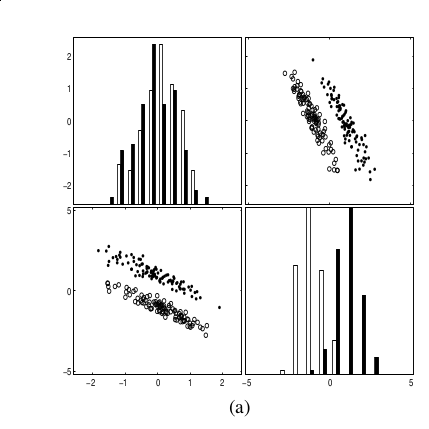
\includegraphics[width=100mm]{../img/guyeli_figure3.png}
\caption{Example of correlated features from the article}
This example has been taken from \citet{GuyEli03}.
\label{fig:guyeli03-figure3}
\end{figure}

There are number of filters differing in the filter condition.
We will discuss mutual information and Chi-square.

\subsubsection{Mutual Information}\label{subsubsec:mi}

As \citet{Hoq14} defines it,
{\bf mutual information}~$I(X, Y)$~is the amount of uncertainty in X due to the amount of knowledge of Y.
{\bf Mutual information} of variables $X$ and $Y$ is defined as:

\begin{equation}
I(X,Y) = \sum_{x,y} p\left(x,y\right)
\log
\frac{p\left(x,y\right)}{p\left(x\right)p\left(y\right)},
\label{eq:mi}
\end{equation}

where $p\left(x, y\right)$ is the joint probability of~$X$ and $Y$ and~$p(x)$~and~$p(y)$~
are marginal probability distributions of the individual variables.

Mutual information can be also expressed as

\begin{equation}
	I(X, Y) = H(X) - H(X|Y),
\end{equation}

\todoB{explain entropy}

where~$H(X)$~is the entropy of~$X$~and~$H(X|Y)$~the conditional entropy.
This way~$H(X)$~expresses the amount of uncertainty of~$X$~and~$H(X|Y)$~what~$Y$~does not say about~$X$.
This supports the intuitive idea that information gain expresses how much information one variable carries about the other one.

Let us demonstrate mutual information on an example.
Suposse we are trying to predict the mood of the examiner for our exam.
We have created two features --- whether it is raining and whether the examiner is hungry.
Mock data is shown in \Cref{tab:mi_ex}.
Now, we want to estimate how good those features are using mutual information.


\begin{table}[h!]
 \center
 \begin{tabular}{lll}
	\toprule
	 \textbf{raining} & \textbf{hungry} & \textbf{mood} \\ 
	 \midrule
	 yes & yes & happy \\
	 no & yes & happy \\
	 no & yes & angry \\
	 no & no & angry \\
	 yes  & no & angry \\
	 \bottomrule
 \end{tabular}
 \caption{Mutual information example}
 \label{tab:mi_ex}
\end{table}

Using \Cref{eq:mi}, MI of variables $\mathit{rain}$ and $\mathit{mood}$ is:


\todoA{this looks ugly}
\begin{equation}
	I(\mathit{rain}, \mathit{mood}) =
	f(yes, happy) + f(no, happy) + f(yes, angry) + f(no, angry),
\end{equation}

where:

\begin{equation}
	f(x, y) = P(rain=x,mood=y)\log\frac{P(rain=x,mood=y)}{P(rain=x)P(mood=y)}
\end{equation}


With the values from \Cref{tab:mi_ex}, we get:

\begin{equation}
	I(\mathit{rain}, \mathit{mood}) =
	\frac{1}{5}
		\log \frac{
	\frac{1}{5}
	}{
	\frac{2}{5}
	\frac{2}{5}
	} +
%
	\frac{1}{5}
		\log \frac{
	\frac{1}{5}
	}{
	\frac{3}{5}
	\frac{2}{5}
	} +
%
	\frac{1}{5}
		\log \frac{
	\frac{1}{5}
	}{
	\frac{2}{5}
	\frac{3}{5}
	} +
%
	\frac{2}{5}
		\log \frac{
	\frac{2}{5}
	}{
	\frac{3}{5}
	\frac{3}{5}
	}
\end{equation}

\begin{equation}
	I(\mathit{rain}, \mathit{mood}) \approx 0.014
\end{equation}

We compute $I(\mathit{hungry}, \mathit{mood})$ in the same way:

\begin{equation}
	I(\mathit{hungry}, \mathit{mood}) =
	\frac{2}{5}
		\log \frac{
	\frac{2}{5}
	}{
	\frac{3}{5}
	\frac{2}{5}
	} +
%
	\frac{0}{5}
		\log \frac{
	\frac{0}{5}
	}{
	\frac{2}{5}
	\frac{2}{5}
	} +
%
	\frac{1}{5}
		\log \frac{
	\frac{1}{5}
	}{
	\frac{3}{5}
	\frac{3}{5}
	} +
%
	\frac{2}{5}
		\log \frac{
	\frac{2}{5}
	}{
	\frac{2}{5}
	\frac{3}{5}
	}
\end{equation}

\begin{equation}
	I(\mathit{hungry}, \mathit{mood}) \approx 0.291
\end{equation}

The mutual information of \textit{hungry} is higher than \textit{raining}.
It intuitively makes sense if we look at the table.
\textit{Hungry} predicts the mood four times out of five correctly.
Especially, when the examiner is hungry, he is always happy.
On the contrary, regardless whether it is raining or not, the examiner
is sometimes happy, sometimes angry.

Once we know how to compute mutual information,
we only need to select the best performing features.
The basic approach is to compute mutual information of each feature and the class label.
Only features exceeding some given threshold are used for training.

There is also an improved algorithm proposed by \citet{Hoq14}.
Instead of choosing all features in one step,
only one feature is chosen any time.
We have two sets; selected ($S$) and candidates ($C$) features.
In the beginning, all features are in $C$.

Every step, we choose one feature from~$C$ and move it to~$S$.
Which feature is chosen depends on two values calculated for each feature from~$C$.
First, feature-class as in the basic approach.
Second, the average of mutual information between the feature and all features from $S$.
We choose such a feature that has the highest feature-class and also lowest average of feature-feature.
This prevents including highly correlated features in~$S$.

Let us demonstrate it on two correlated features~$A$~and~$B$.
Adding~$A$ into~$S$ results in~$B$ having higher average of mutual information with features from $S$.
As such, $B$ is less likely selected in the next steps.

We stop, once the mutual information of the feature chosen from $C$ and the class drops bellow a certain
threshold.
At the end, features from~$S$ are used for classification.
We have not used this approach due to the lack of time and used the basic approach only.


\subsubsection{Chi-square~---~$\chi^2$}

Chi-square test of independence can be thought of
as a measure of lack of the independence between two variables.
As in mutual information,
we will compute a special value for each pair feature-class
and based on some threshold we will choose the most informative features.
We will briefly discuss the idea and present an example.
More detailed description can be found in~\citet{Hugh13}.


Let us demonstrate this with an example.
We have instances of our reviews and we want to test how well
feature \textit{credit card} describes
labels \textit{useful} and \textit{not-useful}.
The feature expresses whether the phrase ``credit card'' is present in the text of a review.
To asses this, we want to compute~$\chi^2$ of the variables~$X$~and~$Y$.
First, representing the feature \textit{credit card}.
Second, the true label.

\Cref{tab:chi_ex} shows example data.
The inner cells express how many instances there are with the given combination of variable values.
The bottom most row and right most column express marginal probability distributions
calculated by the number of samples.
If the variables were truly independent,
we would expect the cells to be 15 and 35 in the first and second row, respectively.
We will introduce a cost function to reflect this
and~$\chi^2$~of the two variables will then be sum of the cost function over all cells.


\begin{table}[h!]
 \center
 \begin{tabular}{ll|r|r|r}
 \cline{3-4}
        &       & \multicolumn{2}{c|}{label} & \\
        \cline{3-4}
        &       & yes        & no            & $P_Y$ \\
        \cline{1-4}
	 \multicolumn{1}{|l|}{credit} & yes   & 25         & 5             & 0.30 \\
        \cline{2-4}
	 \multicolumn{1}{|l|}{card}   & no    & 45         & 25            & 0.70 \\
        \cline{1-4}
		& \multicolumn{1}{l}{$P_X$} & \multicolumn{1}{l}{0.50}       & \multicolumn{1}{l}{0.50}          & 1
 
 \end{tabular}
 \caption{$\chi^2$~Example}
 \label{tab:chi_ex}
\end{table}

Let us have two random variables~$X$~and~$Y$.
Let us define~$O_{x,y}$ and~$E_{x,y}$
as respectively the number of observed and expected instances for~$X=x$~and~$Y=y$.
The value of~$O_{x,y}$~is simply the number of instances.
The value of~$E_{x,y}$ is computed from marginal probabilities.
Namely:

\begin{equation}
E_{x,y} = P_X(X=x) \times P_Y(Y=y) \times n,
\end{equation}

where~$P_X$~and~$P_Y$~are the marginal probabilities of the variables~$X$~and~$Y$
and~$n$~number of all instances.

We define $\chi^2$~of two random variables~$X$~and~$Y$~as:

$$\sum_{x \in X, y \in Y}{\chi^2_{y,x}},$$

where~${\chi^2_{y,x}}$ is $\left(O_{x,y} - E_{x,y} \right)^ 2 / E_{x,y}$.

This corresponds to our intuition.
If the variables are correlated,
the observed values will differ from expected and~$\chi^2$ will by non-zero.
The farther observed value from the expected is, the higher penalization with square.
Also, it is normalized by dividing it in E.

The value of $\chi$ in our example in \Cref{tab:chi_ex}
~is:

\begin{equation}
\chi^2 = 
\frac{\left(25-15\right)^2}{15} +
\frac{\left(5-15\right)^2}{15} +
\frac{\left(45-35\right)^2}{35} +
\frac{\left(25-35\right)^2}{35}
\end{equation}

\begin{equation}
\chi^2 \approx 11
\end{equation}


\subsection{Wrappers}

Description of both variants of wrappers can be found in \citet{GuyEli03}.
More thorough analysis is in \citet{kohavi1997wrappers}.

Unlike filters, wrappers work with subsets of features
and use a classifier to directly asses informativeness of the subset as a whole.
Every subset is classified by the classifier used as a black box
and evaluated by some common evaluation metrics.
The optimal subset is than chosen.
Thanks to this, wrappers are universal and robust.

Also, wrappers can perform a lot better than filters on certain datasets.
Such an example was shown in \Cref{subsec:filters}.

Unfortunately, wrappers tend to be computationally expensive,
because every subset must by classified separately.
In fact, it has been shown it is NP-hard to find optimal solution.
To achieve computational feasibility, various approximation methods has been developed.
These methods allow us to classify only a fraction of subsets
at the cost of losing the guarantee of the optimal solution.
We will describe two variants of greedy search.

\todoB{On the approximability of minimizing nonzero variables
or unsatisfied relations in linear systems --- citation of the NP-hard, otherwise delete} 

\subsubsection{Greedy Search --- Forward Selection}

{\it Forward selection} starts with an empty set and in every step adds a feature which brings the highest increase of performance in the evaluation metrics.
As we said, we use a classifier and some common evaluation metrics to asses the performance.
The score of a candidate feature is then difference between the performance of the classifier trained on the current feature set with this feature and without it.
The feature with highest score is added and the process repeated until the increase in performance is less than a certain threshold. 

\subsubsection{Greedy Search --- Backward Elimination}

{\it Backward elimination} works analogously to forward selection.
We start with the set of all features.
In one step a feature with lowest decrease in score is removed.
This step is repeated until the evaluation drops by more than a given threshold.
This approach may be infeasible for really big data sets, but guarantees to include all useful features of which some may be omitted by forward selection.

\subsection{Embedded Methods}

Embedded methods are part of a classification algorithm itself.
An example can be a decision tree, which takes features that lower the entropy the most first.

\section{Principal Component Analysis}

Principal component analysis is not feature extraction nor selection.
It is rather an intermediate process between feature engineering and training a classifier.

\textbf{Principal component analysis} (PCA) is another way of reducing the number of features used.
Instead of selecting a feature subset, it treats instances as feature vectors.
A \textbf{Feature vector} is a vector wherein each element corresponds to a value of one feature.
The order of features is fixed.
This way we can represent an instance with all its features by a vector.

The idea of PCA is to transform feature vectors into a space of lower dimensionality.
The objective is to retain as much information contained in the vector, while
having lower dimensionality.
Mathematically speaking, the objective is to retain as much variation of variables
as possible and reduce any variable correlation.
The exact description is way beyond the scope of this text.
More detailed explanations can be found in~\citet{Jolliffe02}.

\section{Commonly Used Features}

In this section, we will use some commonly used features and briefly discuss their pros and cons.

\subsection{Bag-Of-Words}
\label{subsec:bow}

Since the information a sentence carries is not contained only in the words, but also in their positions in the sentence, an ideal algorithm would take into account both the words and their positions.
However, working with sentences as a whole is somewhat difficult. Hence, the order of words is often omitted and only the word occurrences matters.
\textbf{Bag-Of-Words} (BOW) encodes this information by mapping every word onto the number of occurrences in the given text.

\subsubsection{TF-IDF}

In a general document, there are many words that are not directly useful.
{\it TF--IDF} is a way to evaluate which words are the most important for individual documents and
choose reduce the number of words used in BOW.

\citet{ramos2003using} Describe using TF-IDF for detecting relevant words.
TF-IDF for text classification is described in \citet{trstenjak2014knn}.
Even though variations for improving performance have been described,
we introduce the basic version of TF-IDF.
More advanced variants can be found in \citet{berger2000bridging} or
\citet{yun2005improved}

The motivation for introducing TF-IDF is well described in \citet{SalBuc88}.
The goal is to select such words for a document
that they will define it well enough, yet leave enough room for describing all relevant documents by the same words.
We will introduce two metrics to convey these two requirements and then use a combination of those two to gain the best results.

First, we will simply use only words occurring frequently enough in a document.
The number of occurrences of a word in a document is referred to as {\it term-frequency}.
Second, we will use {\it inverse-document frequency} (IDF) to skip words such as {\it an}, {\it the} which appear in virtually every sentence and carry very little information.
IDF is indirectly proportional to the number of documents which contain a given word.
Thanks to this, words like articles will be given very little weight.

There are many implementations of this general idea.
We will explore the implementation described in \citet{Ramos03}.
Given a set of documents~$D$
we can calculate TF-IDF for word~$w$ in an individual document~$d$ as:

\[
	w_d = TF \times IDF = f_{w, d} \times \log \left( \frac{\abs{D}}{f_{w,D}}  \right),
\]

where $TF = f_{w, d}$ is the number of times~$w$~occurred~$d$ and
IDF corresponds to $\log \left( \frac{\abs{D}}{f_{w,D}}  \right)$ for $\abs{D}$ being the total number of documents and $f_{w, D}$ the number of documents containing~$w$.

Let us explore how the value changes with different variable values.
For such words that $\abs{D} \sim f_{w, D}$ the value of logarithm is very low and so is the importance of the words.
This is desired behaviour because words that occur in virtually every document  are not very useful.
On the other hand, words having $f_{w,d}$ large and $f_{w,D}$ small are given much higher importance.
This is again desired, because these words occur relatively often in the given document and not so often in the document set overall.


\subsection{N-grams}

When using BOW, we can potentially loose useful information conveyed in the word order.
Unfortunately, it is often computationally infeasible to retain the complete order.
To find a balance, N-grams try to convey the order only partially.
\textbf{N-gram} is simply a sequence of items, in our case words. The~$N$~refers to the length of the sequence.
The longer a sequence is the more order is preserved at higher computational cost.
Bigrams and trigrams (pairs and triples) are most commonly used.

\todoB{- choose words with highest information gain; as in McCallum Event models}

\subsection{Word Embeddings}
\label{subsec:wordembed}

Word embeddings is another way to convert words into features.
\citet{LeGo14} describe {\bf word embedding} as a mapping of every word to a vector in~$R^d$.
This is also sometimes referred to as \textit{distributed word representation}.
This mapping is obtained by using a big corpus of data and optimizing some cost function on it.

\citet{Mik13} showed that if parameters are set carefully, word embeddings conveys both semantic and syntactic information.
First, similar words are mapped to similar vectors. So we can measure a sort of synonymity.
Not only that, but it also conveys relationships between words.
An example is singular vs plural.
Let~$x_{w}$ be the vector of the word~$w$.
They showed that $x_{apple}-x_{apples} \sim x_{car}-x_{cars}$.
Even more complicated relations like $x_{king} - x_{man} + x_{woman} \sim x_{queen}$ were shown.
They use this property to solve word analogies in the form {\it a is to b as c is to \_\_\_}.


\subsection{Entities}

Named entity is any group of words belonging together having a particular meaning.
The words does not necessarily be adjacent.
In the text bellow, there are among other entities \textit{limited hour} and \textit{good fare}.

\begin{code}
Another case of the Emperor's New Clothes.
Someone of the artsy set decided that this relatively good
but overpriced fare was great pizza and all the lemmings followed suit.
\end{code}

For extracting entities, we used NLP analysis as described in \Cref{app:geneea}.

 %\todoB{- filter them based on the~geneea value of importance}

 %\todoA{- occurrences - pick only the~most frequent}

\subsection{Sentiment Analysis}

\textbf{Sentiment analysis} (also referred to as \textit{opinion mining}) is described by \citet{melville2009sentiment} 
as a task of identifying writer's feeling expressed in a text about a topic.
\textbf{Sentiment} is then the particular mood of a text.

Examples of texts with different sentiments are bellow.

Negative:

\begin{code}
The pizza was horrible.
\end{code}

Neutral:

\begin{code}
They offer pizza.
\end{code}

Positive:

\begin{code}
The pizza was delicious.
\end{code}

A text can of course contain different moods.
The example bellow is negative in the first part and positive in the second part.

\begin{code}
The place is horrible, but the pizza was great.
\end{code}

We use negative, neutral and positive sentiment extracted from the reviews by the NLP analysis.
The sentiment is used as a direct feature.

The actual sentiment analysis is beyond the scope of this thesis.
\citet{kaushik2014scalable} lists two main approaches; machine learning and lexicon based solutions.
Machine learning is well described in \citet{melville2009sentiment} or \citet{xia2011ensemble}.

\subsection{Cosine Similarity}

\textbf{Cosine similarity} is a measure of similarity between two feature vectors.
It is the angle between the two vectors.
The cosine similarity of vectors~$v$~and~$w$~is:

\[
	\mathit{similarity} = \cos\left(\theta\right) = \frac{v \cdot w}{\|v\| \| w \|}
\]

Usually, one takes a sample from the data and when classifying an instance,
cosine similarities to all instances in the sample are computed.
The feature suggests that an instance has the label with the label of the closest instance.

Cosine similarity is well measured with number of proposed extensions.
More precise description with improvements over the basic variant can be found
in \citet{li2013distance} or \citet{mikawa2011proposal}.


\subsection{Hand Crafted Features}

\subsubsection{Spell check}

We also tried to measure typos in the review.
The hypothesis was that reviews with many typos may be less useful,
because the reviewer apparently did not spend much time writing it.
We tried to split features into two groups --- with and without typos.

The method we used was not perfect.
We use the package aspell.\footnote{\url{http://aspell.net}}
It compares words against dictionary and report any not-found words.
This way, it can report words that are not typos and are not present in the dictionary.
Also, it may not report words that are incorrect in a particular context,
but alright in another (such as \textit{you're} vs \textit{your}).

We are also aware, that reviews contain many special words such as names of food that
are technically from a different language, but are use in English unchanged.
We ignored these problems,
because we did not need the exact value of typos,
but whether it is bellow and above a certain threshold.


\subsubsection{Review length}

Another hand crafted feature was a review length.
It is simply the number of words as returned by the already described twitter tokenizer.
Again, we clustered values into groups to get binary or ternary features.


\subsection{non-textual features --- metadata}

Sometimes it may be necessary to use metadata
if the text itself does not contain enough information.
The exact usage will depend on the task.
We used metadata mostly for filtering out restaurants without enough data.
The only feature we tried to extract from metadata was the number of stars the review gives.
We tested two approaches.
First, a simple feature expressing how many stars were given.
Second, we tried to have a feature \textit{extreme stars}.
This feature is binary being one if the user gave 1 or 5 stars;
zero otherwise.

We were hoping that reviews with 1 or 5 stars may express very strong opinion
and as such are more likely to be useful.

In this chapter, we outlined how to extract and select features.
Finally, we introduced concrete features we used for classification.

\chapter{Feature Engineering}

\todoA{FEATURE SELECTION FOR
KNOWLEDGE DISCOVERY AND
DATA MINING
Huan Liu
Hiroshi Motoda}

\todoA{What is a feature?? - ref from previous part}

\todoA{do these two paragraphs need citation too?}

Features are divided by their values into three categories~---~nominal, ordinal and continuous. Nominal features are discrete and their values do~not convey any relationship. When a~feature is ordinal, it means it is discrete and also convey ordering of the values. Continuous feature is then any real-valued variable.

In this text we will deal with nominal and ordinal only. The simplest way to treat ordinal features is to omit the order. This of course loses information conveyed in this ordering, but will allow us easier feature manipulation.

\section{Commonly Used Features}

\subsection{bag-of-word (BOW)}

\subsubsection{td-idt}

\todoA{source: Using TF-IDF to Determine Word Relevance in Document Queries - downloaded}

\subsubsection{*-gram}




\subsection{Singular Value Decomposition (SVD/PCA)}

\subsection{Word embeddings}

\subsection{hand crafted features}

\subsection{non-textual features --- metadata}



\section{Extraction}

Too many feature -> extraction, selection



\section{Selection}

Machine learning is used in contexts where the true natural and inner logic of~data is~not known. Therefore it is difficult to intuitively select only useful features. Having fewer features which are informative enough leads to three direct benefits.

Trained model is far less complex and as~such easier to~interpret. The~model also generalises better, because the~risk of overfitting is lower. Overfitting happens when the~model recognises irregularities in training data and classifies individual already seen instances, whereas it should approximate the~original model to~be able to~classify unseen instances. Lastly, fewer features result in shorter training time.

Three types of feature selection are generally recognised.



\subsection{Filters}

Filters are popular, because their time complexity is linear in the~number of~features. However, the feature selection may~not be optimal, because neither the~used classificator nor feature correlation is taken into account. When there are highly correlated features, it is unnecessary to choose all of them, because the information conveyed in some may be inferred from others. However, any filter will choose all of them, because filters consider features independently of each other.

Filters work with individual features independently of any supervised classification algorithm. Each feature is used or omitted based on the filter condition. There are number of filters differing in the filter condition.

\subsubsection{PMI}

\subsubsection{MI}

\subsubsection{$\chi^2$}




\subsection{Wrappers}

Unlike filters, wrappers work with subsets of features. Every subset is classified by a classificator used as a black box and then evaluated by some common evaluation metrics. The optimal subset is than chosen. Thanks to this, wrappers are universal and robust.

Furthermore, wrappers can perform a lot better than filters on certain datasets. Such a~case is documented by \citet{GuyEli03} in~\ref{guyeli03-figure3}. The bottom left graph shows the original data and the~top left shows projection onto only one axis. It is clear that one variable cannot be sufficient for separating the clusters. However, if we project the data onto a combination of the two axis, the clusters can be at least partially separated as can be seen in the right part of the figure.
 
 \todoA{citation and vector}

\begin{figure}[ht]\centering
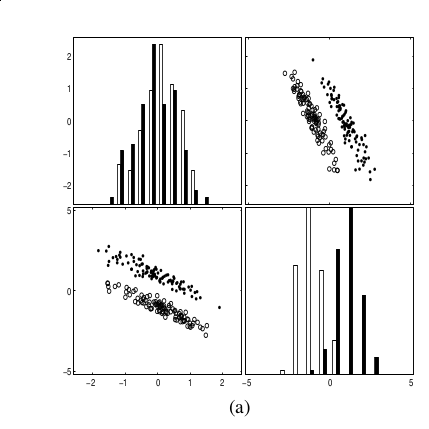
\includegraphics[width=100mm]{../img/guyeli_figure3.png}
\caption{Example of correlated features from the article}
\label{guyeli03-figure3}
\end{figure}

Unfortunately, wrappers tend to be computationally expensive, because every subset must by classified separately. In fact, it has been shown it is NP-hard to find optimal solution. To achieve computational feasibility various approximation methods has been developed. These methods allow us to classify only a fraction of subsets at the cost of losing the guarantee of the optimal solution. We will describe two variants of greedy search.

\todoB{On the approximability of minimizing nonzero variables
or unsatisfied relations in linear systems --- citation of the NP-hard, otherwise delete} 

\subsubsection{Greedy Search --- Forward Selection}

{\it Forward selection} starts with an empty set and in every step adds a feature which brings the highest gain in the evaluation metrics. The feature is selected by adding all of them to the current  subset and evaluating it. The step is repeated until the increase in performance is less than a certain threshold. 

\subsubsection{Greedy Search --- Backward Elimination}

{\it Backward elimination} starts with the set of all features. In one step every feature is removed from the subset and this new subset is than evaluated. The feature which decreased the evaluation the least will be removed. This step is repeated until the evaluation drops by more than a given threshold. This approach may be infeasible for really big data sets, but includes all useful features of which some may be omitted by forward selection.




\subsection{Embedded Methods}

Embedded methods are part of a classification algorithm itself. An example can be a decision tree, which takes features that lower the entropy the most first. More on this in particular algorithms.

\todoA{The last sentence should be removed if there are no such algos in this doc.}




\chapter{The Software Project Architecture}\label{chap:arch}

In this chapter, we outline the conceptual design of the software package.
We describe individual parts and how they interact.
More thorough description with implementation details and configuration can be found in \Cref{app:techn}.


The software package was designed and developed with extensibility in mind.
It allows easily adding new features, specifying different subsets of data and converting them into various format without breaking older experiments.
Various libraries are utilized for both higher performance and easier maintainability.
Abstract classes are utilized for defining clear API and allow easy addition of new algorithms.

A special configuration file is utilized allowing to change the behaviour without touching the code base.
All classes and files have documentation strings which should be sufficient for detailed understanding.
In this chapter, we only describe the high-level overview.

A conceptual overview is outlined in \Cref{fig:conceptual_design}.
The flow of the programme is top to bottom.
Ellipses represent processes, rectangles data and cut rectangles input data.
The output is represented by \textit{result}.

First, unused reviews are dropped resulting in \textit{filtered reviews}.
Filtered reviews are added the information about the businesses they belong to in \texttt{join}.
The result is stored in the \textit{instance file}.

In addition to the provided data, external text analysis is used.
Entities and sentiment are extracted from all reviews and
subsequently not used reviews are dropped resulting in \textit{filtered entities and sentiment}.

The two files \textit{instance file} and \textit{filtered entities and sentiment} 
are used for generating instances with all necessary data represented by \textit{full instances}.
Full instances are split into pairs of training and testing sets for k-fold cross validation.

Next, \textit{experiments file} is loaded.
Information about classifier configuration is used to generate samples from \textit{train and test sets pairs}.
The samples have exactly the needed features for the particular classifier and necessary preprocessing is done
resulting in \textit{preprocessed instances}.

Preprocessed instances are used for training a model which is used for predicting test set.
The predictions are used for evaluation performance.
Evaluation results are saved into output files as defined in \textit{graphs specification} extracted from
the \textit{experiments file}.


\begin{figure}[ht]
    \centering
	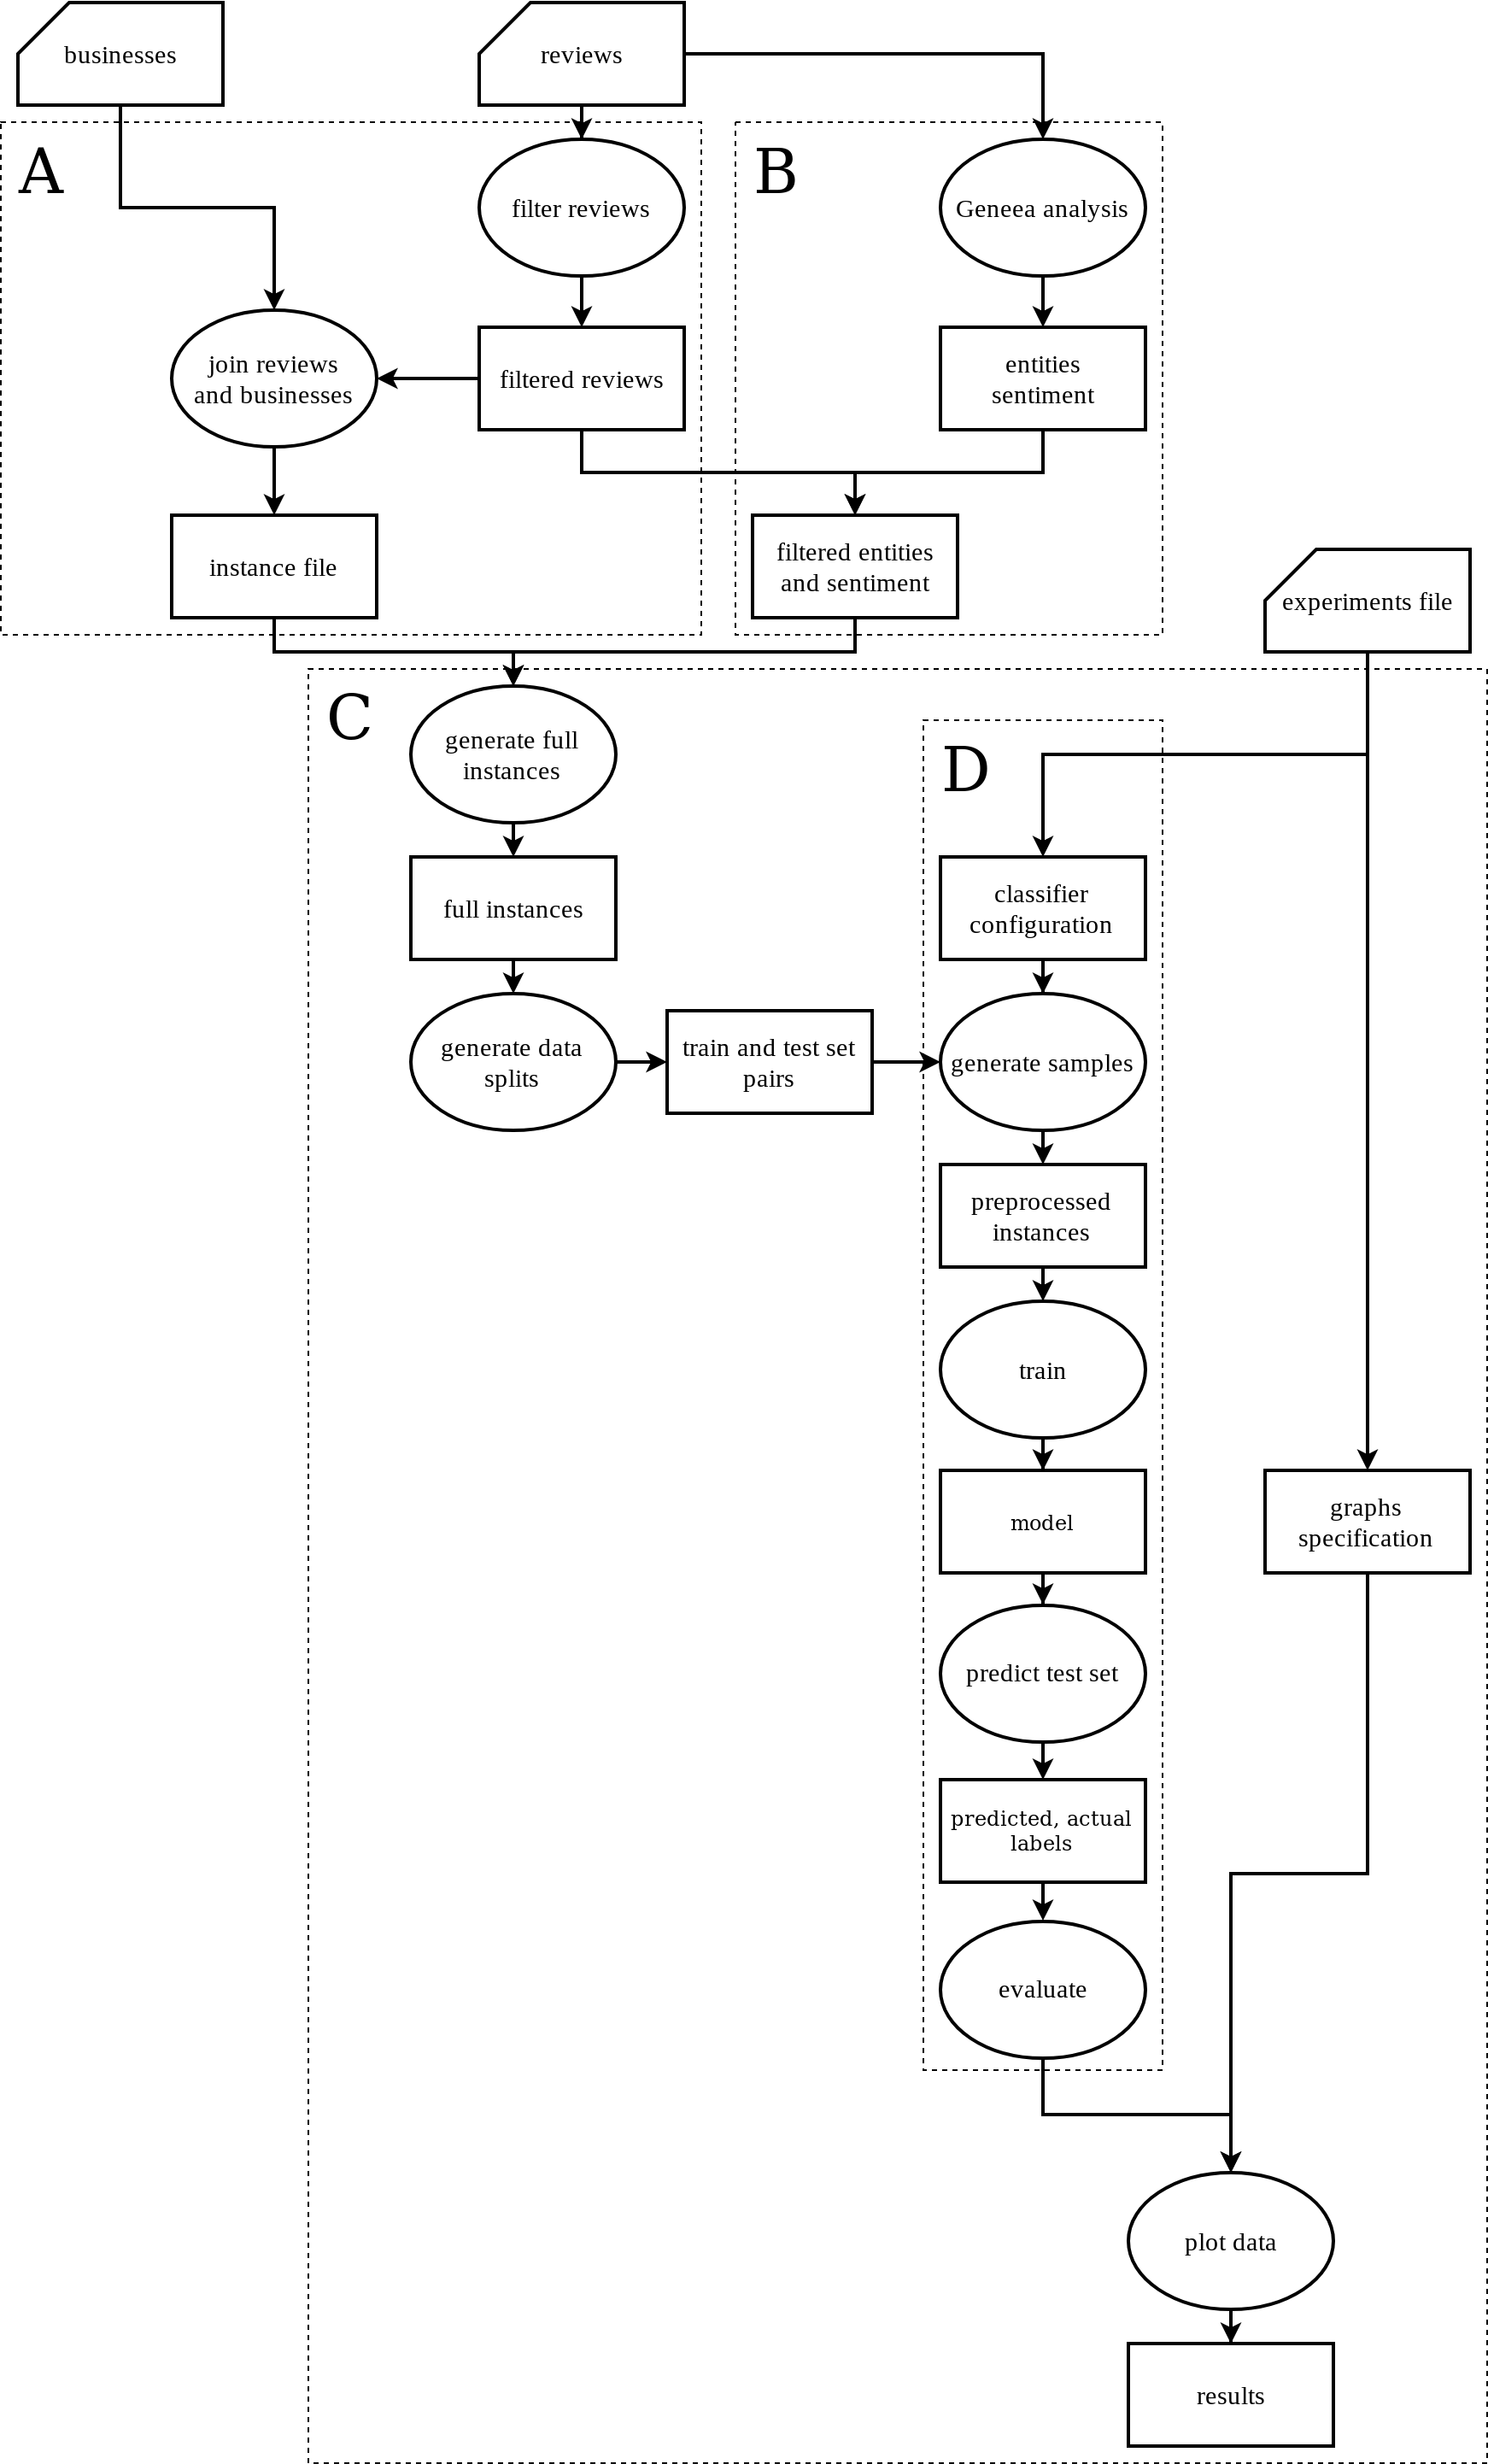
\includegraphics[width=\textwidth]{figures/conceptual_design.png}
	\caption{Conceptual Design}\label{fig:conceptual_design}
\end{figure}






\section{Parts Overview}

The project is implemented in three separate parts as shown in \Cref{fig:arch_process}.
\texttt{Prepare data} creates the instances file and corresponds to rectangle A in \Cref{fig:conceptual_design}.
\texttt{Add NLP analysis} corresponds to rectangle B --- it creates filtered entities and sentiment.
The last part \texttt{Run experiments} does the entire training, evaluating and creating statistics process.
It is represented by rectangle C.
Subset of the last part is devoted to running the experiments; \texttt{run experiments} corresponds to rectangle D.

We describe each part in a separate subsection.

\begin{figure}[ht]
	\centering
	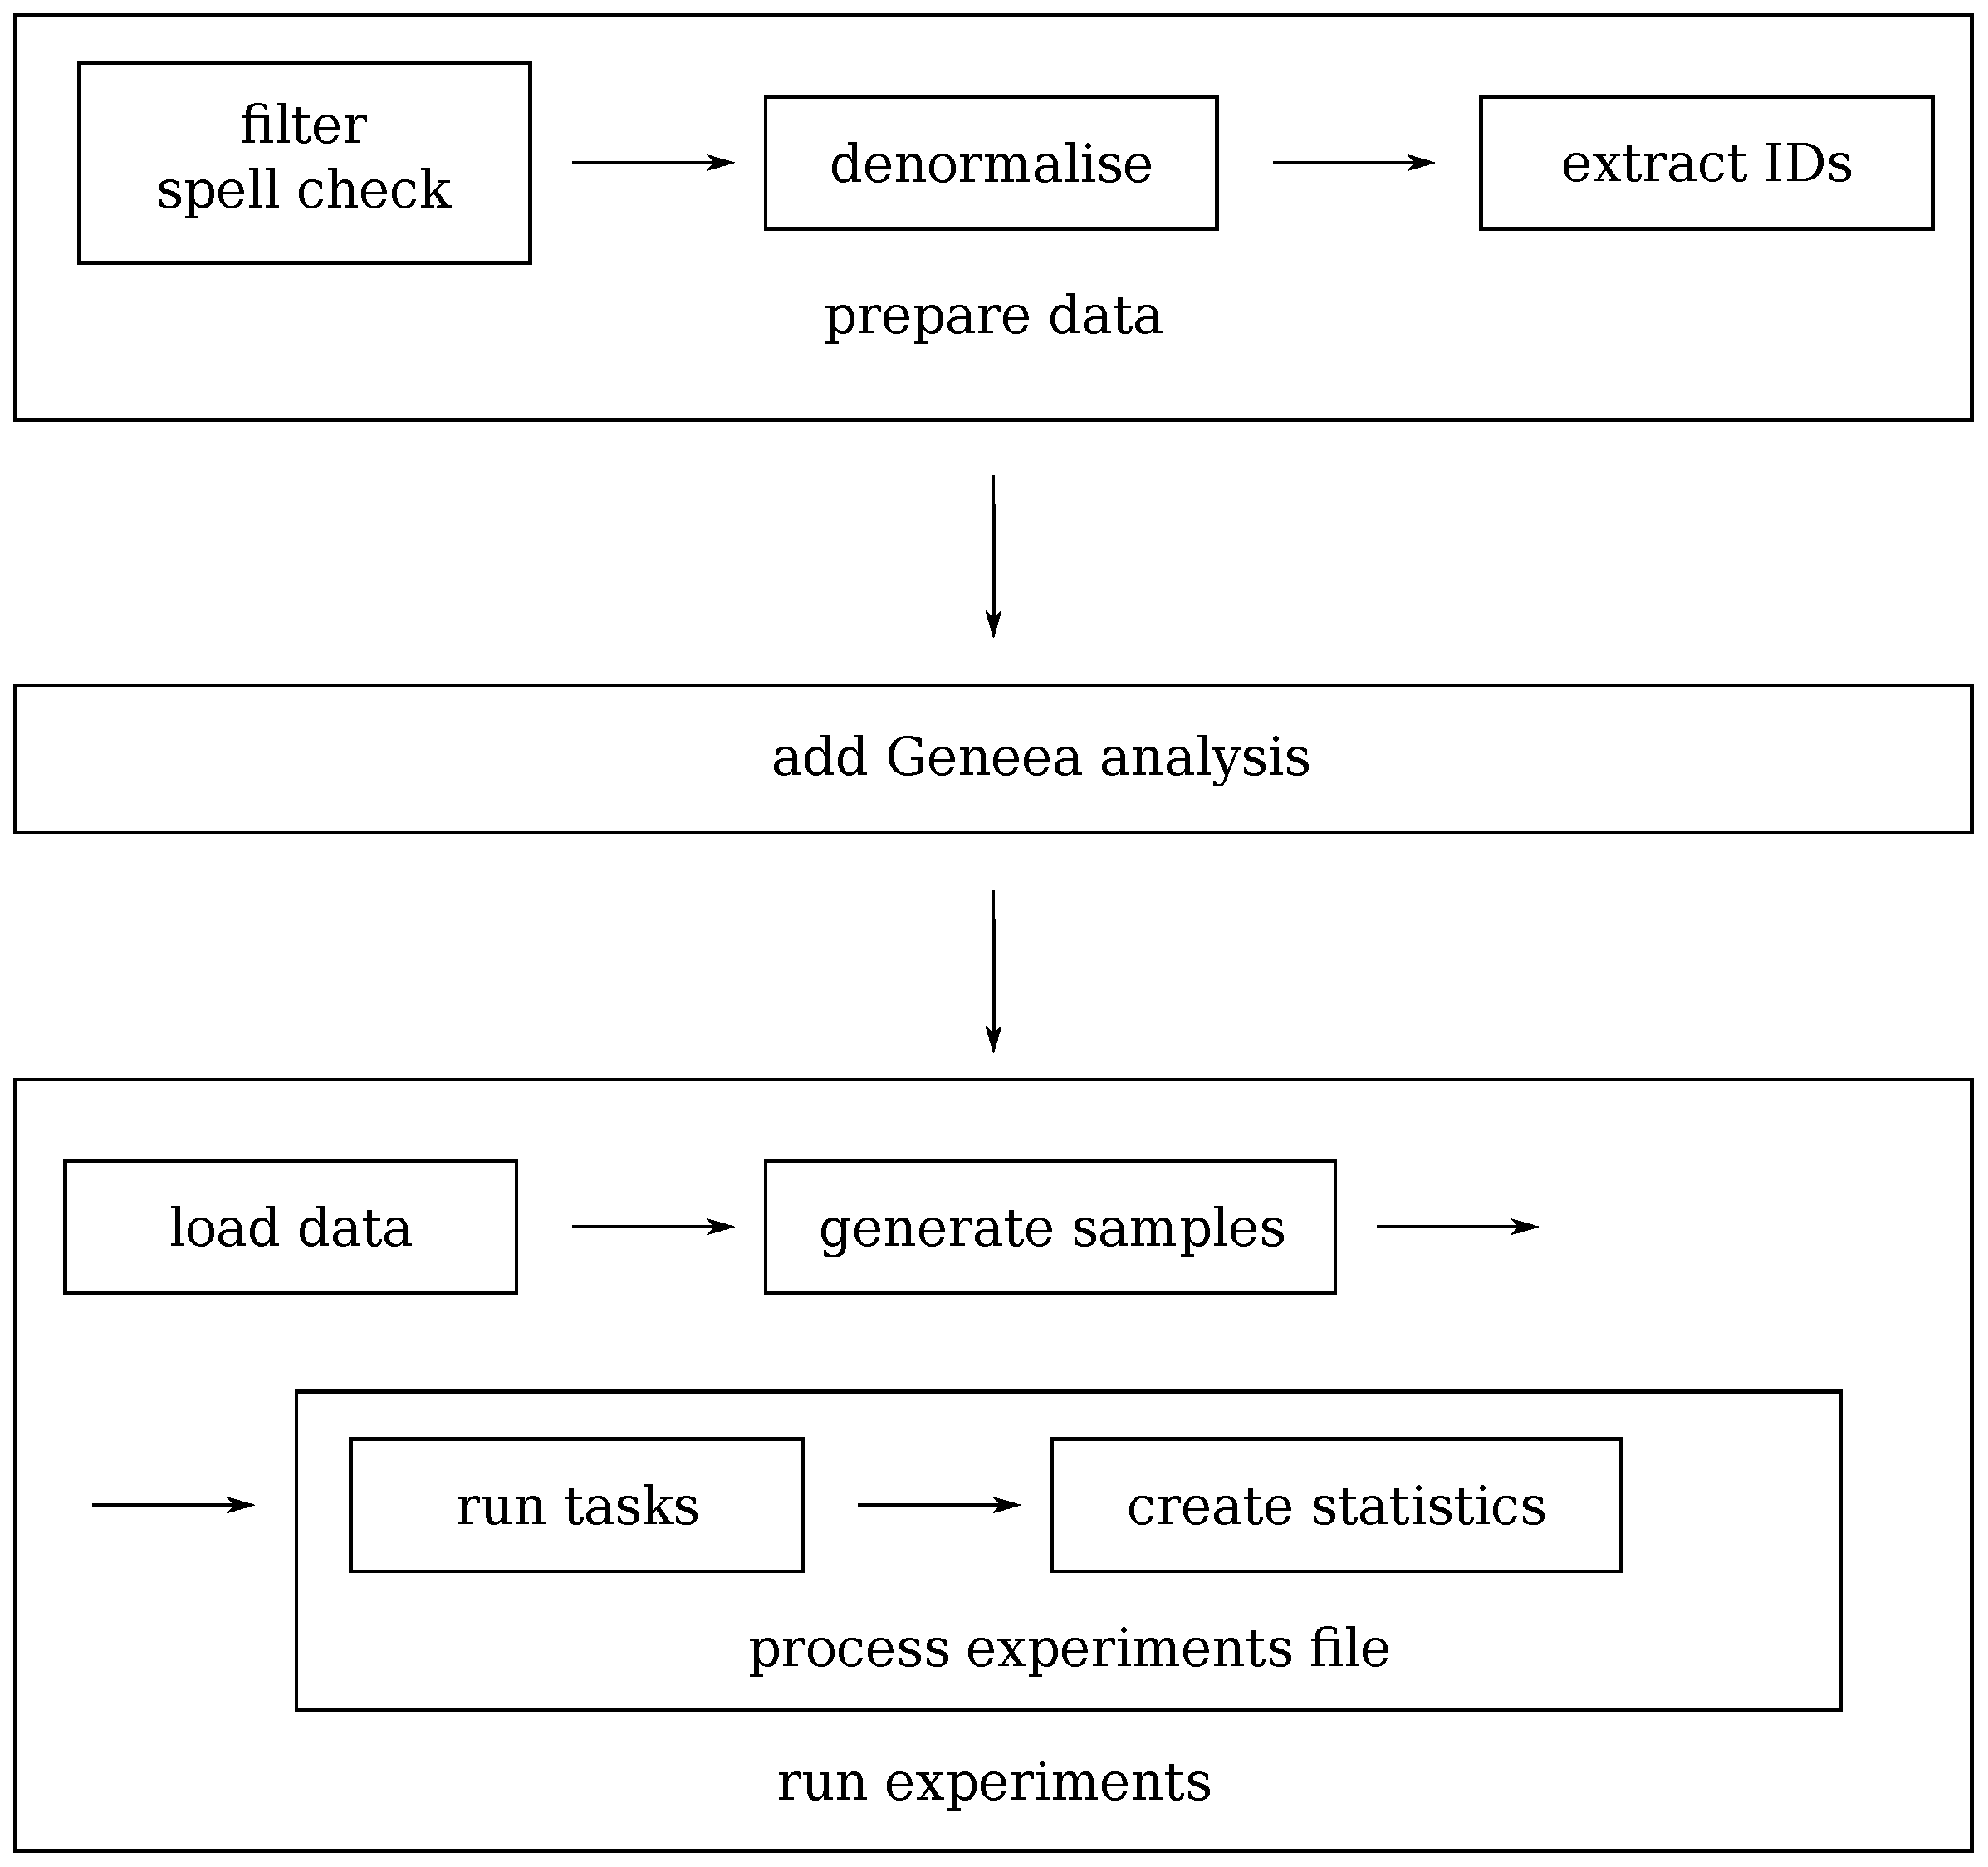
\includegraphics[width=10cm]{figures/arch_process.eps}
	\caption{Architecture Design}\label{fig:arch_process}
\end{figure}


\subsection{Data Preparation} 

All scripts for preparing data are in the folder \texttt{denormalization}.
These scripts take the dataset and produce an instance file.
Filtering of reviews as specified in \Cref{sec:filter} is done.
Because reviews are processed through the spellchecker for filtering,
the output is added into data as a byproduct.
In \texttt{denormalize}, businesses are joined.

At the end, in addition to the instance file, ID file is also created.
It contains extracted IDs from the instance file.
This is used to tell the NLP analyzer what reviews are needed to save bandwidth,
because the analysis is performed on a remote server.

\subsection{NLP Analysis}

NLP analysis uses external tools for extracting more linguistics features.
Thorough description can be found in \Cref{app:geneea}.
The analysis extracts entities and sentiment from all reviews.
Subsequently, it takes filtered reviews in the form of ID file to drop all unnecessary data.
The result is stored in a file, which has to be transferred to the local computer in order to be able to continue with the next part.





\subsection{Run Experiments}

This entire part is handled by \texttt{process\_data.py}, which executes other parts of the code.
Loading data and generating samples is handled by \texttt{load\_data.py}.
Preprocessing is defined in directory \texttt{preprocessors} and classification models in \texttt{classifiers}.
Finally, creating statistics is handled by \texttt{my\_statistics.py}.


\subsubsection{Load Data}

The \textit{instance} and \textit{filtered entities and sentiment} files are loaded and
converted into full instances in memory.
This is handled by class \texttt{Data}.
Subsequently, splits are generated and stored in an instance of \texttt{Sample}.
Splits are still raw data, features are generated in the next step.

\subsubsection{Generate Samples}

When \texttt{process\_data.py} loads classifier configuration,
it uses the loaded instances to generate features for the train and test sets.

\subsubsection{Run Experiments}

Running experiments is implemented as a pipeline being fed with the generated sets and outputting predicted labels.
The units of the pipeline are preprocessors (implemented as children of \texttt{preprocessors/preprocessingbase.py}) and a classifier (a child of \texttt{classifiers/classifierbase.py}).
The pipeline is first fed with training data to built a model.
Subsequently, testing data is passed and predicted labels are stored.

The predicted labels are compared to the actual labels and several evaluation metrics are calculated.
Those are stored in an instance of \texttt{DataGraph}, which serves as a buffer until all results are gathered.

\subsubsection{Create Statistics}

When all experiments are run, graph specification is read.
Data from \texttt{DataGraph} is used to plot graphs as per the specification.
An instance of this class is passed to \texttt{Statistics},
which handles the actual data plotting and writing to files.

In this chapter, we covered the conceptual design of the project.
In the following chapter, we discuss the dataset.

\chapter{Conducted Experiments}\label{chap:exp}

In this chapter, we outline all experiments and discuss the results.
We end up with two best performing models --- Na\"{\i}ve Bayes and decision tree.
Maybe somewhat surprisingly, those models do not make use of any word features,
but exploit only high-level features.

Our original intention was to try all combinations of features, feature selection and classifiers.
However, this turned out to be computationally infeasible.
Instead, we tried promising subsets by choosing the best variant out of each round.

The final dataset used for experiments contains  64,550 instances.
We used 10-fold crossvalidation --- each split had
58,095 training and 6,455 testing instances.
The exact format of the dataset can be found in \Cref{chap:dataset}.

We report accuracy and f-measure.
Because every classifier was trained and tested 10 times,
we report the arithmetic mean as the representative value of the classifier
together with minimum, maximum and standard deviation.
As it can be seen from the tables bellow, 
the values were fairly stable with low standard deviation and
as such should be reasonably reliable.

We performed the analysis in five rounds.
We report f-measure and accuracy of all models to retain comparability even throughout rounds.
Each round focuses on a different variable as listed bellow:

\begin{enumerate}
	\item baseline
	\item feature sets with Na\"{\i}ve Bayes
	\item feature selection algorithms
	\item classifiers
	\item size of training data
\end{enumerate}


\section{1st round --- Baseline}

In this round, we ran zero-R and one-R to get an idea about the problem.

Zero-R achieves accuracy of 70\% as reported in \Cref{tab:base_perf}.
This is in compliance with the label distribution,
because the dataset contains approximately the same proportion of not-useful instances.
One-R raises this performance a bit to 73\%.

Because zero-R assigns all instances label \textit{not-useful},
there are no true positive instances.
Hence precision and recall are zero.
For this reason, f-measure is undefined for zero-R.
We can take one-R for f-measure baseline (56\%).

\begin{table}[h!]

\centering
\begin{tabular}{lr@{~}r@{~}rr@{~}r@{~}r}
\toprule
\textbf{name}	& \multicolumn{3}{c}{\textbf{f-measure}} & \multicolumn{3}{c}{\textbf{accuracy}} \\
\midrule
zero-R & \multicolumn{3}{c}{N/A} & 0.70 & (0.69, 0.70) & $\pm$ 0.004 \\
one-R & 0.56 & (0.54, 0.58) & $\pm$ 0.012 & 0.73 & (0.72, 0.74) & $\pm$ 0.005 \\

\bottomrule
\end{tabular}

\caption{Performance of Feature Selections}\label{tab:base_perf}
All reported values are in the format `arithmetic mean (min, max) $\pm$ standard deviation'.
\end{table}

\section{2nd round --- Features}

In this round, we run Na\"{\i}ve Bayes with different sets of features.
Configurations with results are shown in \Cref{tab:feat_perf}.
Names refer to feature sets.
\textbf{\{uni,bi\}grams} and \textbf{\{uni,bi,tri\}grams} are listed n-grams together.
\textbf{basic} is STARS, REVIEWLEN, SPELLCHECK and COSINESIM.

We can clearly see that none of the feature set brought desired improvement.
Only feature set \textbf{basic} brought a 3 percent improvement in f-measure.
Other sets brought immense deterioration.
Any combination of \textbf{Bigrams} or \textbf{TF-IDF} decreased the accuracy by at least 30\%.
This is probably due to overfitting.
The feature sets contains so many features, that our model learnt to recognise
irregularities in the data.
This claim supports a brief analysis of the features showing that
even words like `in', `to' or `that,' which clearly carry no information about usefulness.
It is interesting to note that f-measure did not suffer from such a big decrease.



\begin{table}[h!]

\centering
\begin{tabular}{lr@{~}r@{~}rr@{~}r@{~}r}
\toprule
\textbf{name}	& \multicolumn{3}{c}{\textbf{f-measure}} & \multicolumn{3}{c}{\textbf{accuracy}} \\
\midrule
unigrams& 0.47 & (0.46, 0.48) & $\pm$ 0.007 & 0.30 & (0.29, 0.32) & $\pm$ 0.006 \\
tfidf& 0.47 & (0.46, 0.48) & $\pm$ 0.007 & 0.30 & (0.29, 0.32) & $\pm$ 0.006 \\
\{uni,bi\}grams	& 0.47 & (0.46, 0.47) & $\pm$ 0.005 & 0.30 & (0.30, 0.31) & $\pm$ 0.004\\
bigrams & 0.47 & (0.46, 0.47) & $\pm$ 0.005 & 0.31 & (0.30, 0.31) & $\pm$ 0.005			\\
entities & 0.48 & (0.47, 0.49) & $\pm$ 0.005 & 0.35 & (0.34, 0.36) & $\pm$ 0.005		\\
\{uni,bi,tri\}grams & 0.47 & (0.46, 0.48) & $\pm$ 0.008 & 0.30 & (0.29, 0.32) & $\pm$ 0.007	\\
trigrams & 0.47 & (0.46, 0.49) & $\pm$ 0.008 & 0.32 & (0.31, 0.33) & $\pm$ 0.006		\\
cosine\_sim & \multicolumn{3}{c}{N/A} & 0.70 & (0.69, 0.70) & $\pm$ 0.006		\\
\textbf{basic} & 0.59 & (0.58, 0.60) & $\pm$ 0.005 & 0.71 & (0.71, 0.72) & $\pm$ 0.004		\\
basic+bigrams & 0.48 & (0.47, 0.49) & $\pm$ 0.007 & 0.35 & (0.34, 0.36) & $\pm$ 0.006		\\
basic+tfidf & 0.48 & (0.47, 0.50) & $\pm$ 0.007 & 0.36 & (0.35, 0.37) & $\pm$ 0.006			\\
\textbf{basic+entities} & 0.55 & (0.54, 0.56) & $\pm$ 0.008 & 0.54 & (0.53, 0.55) & $\pm$ 0.006		\\
\bottomrule
\end{tabular}


\caption{Performance of Feature Configurations}\label{tab:feat_perf}
All reported values are in the format `arithmetic mean (min, max) $\pm$ standard deviation'.
\end{table}


\section{3rd round --- Feature Selection}

In this round, we compare three different methods of feature selection.
The attempt is to avoid the overfitting described in the previous section.
We use features \textbf{basic+entities} and Na\"{i}ve Bayes.
We run PCA with 100 dimensions as recommended by scipy documentation.
For mutual information and chi square, we choose top 1000 features.

From \Cref{tab:sel_perf}, we can see that both mutual information
and chi-square improved the accuracy to 58\% and f-measure even to the original
0.56 from the baseline.
Choosing the threshold for the number of features more carefully could improve the results even further, possible above the performance of the baseline.
We have not analyzed this due the lack of time.

PCA decreased the performance by a significant margin.
This could be due to non-optimal parameters, which
again could be improved by more careful analysis.

\begin{table}[h!]

\centering
\begin{tabular}{lr@{~}r@{~}rr@{~}r@{~}r}
\toprule
\textbf{name}	& \multicolumn{3}{c}{\textbf{f-measure}} & \multicolumn{3}{c}{\textbf{accuracy}} \\

\midrule
basic+entities & 0.55 & (0.54, 0.56) & $\pm$ 0.008 & 0.54 & (0.53, 0.55) & $\pm$ 0.006		\\
\textbf{basic+entities[MI]} & 0.56 & (0.55, 0.57) & $\pm$ 0.007 & 0.58 & (0.57, 0.60) & $\pm$ 0.008 \\
\textbf{basic+entities[CHI]} & 0.56 & (0.55, 0.57) & $\pm$ 0.007 & 0.58 & (0.57, 0.59) & $\pm$ 0.007 \\
basic+entities[PCA] & 0.47 & (0.46, 0.48) & $\pm$ 0.007 & 0.30 & (0.3, 0.31) & $\pm$ 0.006 \\


\bottomrule
\end{tabular}

\caption{Performance of Feature Selections}\label{tab:sel_perf}
All reported values are in the format `arithmetic mean (min, max) $\pm$ standard deviation'.
\end{table}

\section{4th round --- Classifiers}

In the fourth round, we decided to try different classifiers as opposed to the previously used Na\"{\i}ve Bayes.
We used the following classifiers and features:

\begin{itemize}
\item Na\"{\i}ve Bayes; \textbf{basic}
\item FastText; raw text
\item decision tree; \textbf{basic}
\end{itemize}

Na\"{\i}ve Bayes was chosen the best performing data set.
Fast Text is designed for working with raw text.
Decision tree tends to suffer from overfitting when too many features are used.
Also, the training time increases significantly with the number of features,
because mutual information needs to be computed for all features in all nodes.
Therefore, we used only feature set \textbf{basic}.

The results can be seen in \Cref{tab:clsf_perf}.
The performance of FastText was comparable to Na\"{\i}ve Bayes on \textbf{basic+entities}.


The best performance in accuracy was achieved by decision tree.
It improves the previous top performing one-R by 3\%, but decreasing the f-measure.
This is a reasonable result, since one-R is a special simpler case of decision tree.
The best performing model in terms of f-measure is Na\"{\i}ve Bayes.


\begin{table}[h!]

\centering
\begin{tabular}{lr@{~}r@{~}rr@{~}r@{~}r}
\toprule
\textbf{name}	& \multicolumn{3}{c}{\textbf{f-measure}} & \multicolumn{3}{c}{\textbf{accuracy}} \\
\midrule

Na\"{\i}ve Bayes & 0.59 & (0.58, 0.60) & $\pm$ 0.005 & 0.71 & (0.71, 0.72) & $\pm$ 0.004		\\

FastText & 0.53 & (0.52, 0.54) & $\pm$ 0.009 & 0.55 & (0.54, 0.57) & $\pm$ 0.008 \\
\textbf{Decision tree} & 0.52 & (0.49, 0.54) & $\pm$ 0.012 & 0.74 & (0.73, 0.74) & $\pm$ 0.004 \\

\bottomrule
\end{tabular}

\caption{Performance of Different Classifiers}\label{tab:clsf_perf}
All reported values are in the format `arithmetic mean (min, max) $\pm$ standard deviation'.
\end{table}


\section{5th round --- Training Size}

Lastly, we perform learning curves analysis as described in \Cref{sec:lcurves}.
Each phase of 10-fold crossvalidation produces training and testing set.
The testing set is the same for all sizes of the training set.
For the training set, subsets of the original are used in such a way that 
all smaller sets are proper subsets of any bigger.

The graphs bellow show both performance of the subset of the training set and of the full testing set.
The x axis is log scaled.
Some values of f-measure for very small sets were ignored for the same reason as with zero-R.
It is undefined as there are no true positives.

We report the two best performing models from the previous round -- Na\"{\i}ve Bayes and decision tree
with feature set \textbf{basic}.

As we can see in \Cref{fig:l_curves2_accuracy} and \Cref{fig:l_curves2_f_measure}, Na\"{\i}ve Bayes performs comparably the same on both the training and testing sets when trained
on already only as many as 100 instances.
It is very likely to generalise well as the performance is virtually identical.
Also, the performance stabilizes well as the minimal and maximal values are very close to the mean.

It is worth noting that decision tree achieves comparable performance as can be seen in
\Cref{fig:l_curves3_accuracy} and \Cref{fig:l_curves3_f_measure}.
However, it needs at least 10 000 instances to achieve so.
Na\"{\i}ve Bayes is a clear winner here as it needs a lot less instances.
It would be beneficial to plot learning curves for other models,
because it could show the reasons why our more sophisticated models with
more features performed significantly worse.
However, due to the computing complexity, we did not analyse it.
It can be the subject of further research.

From the numbers, it is clear that our models did not perform significantly better than the baseline model.
Even our best performing models achieved accuracy of only approximately 70\% which can be accomplished by labelling all instances as not-useful.
The reason could be there is not enough information in the reviews to predict
 usefulness, the inner dependency is much more complicated than what can be conveyed by our simple models or the number of useful likes is not a representative metrics.



\begin{figure}[h]\centering
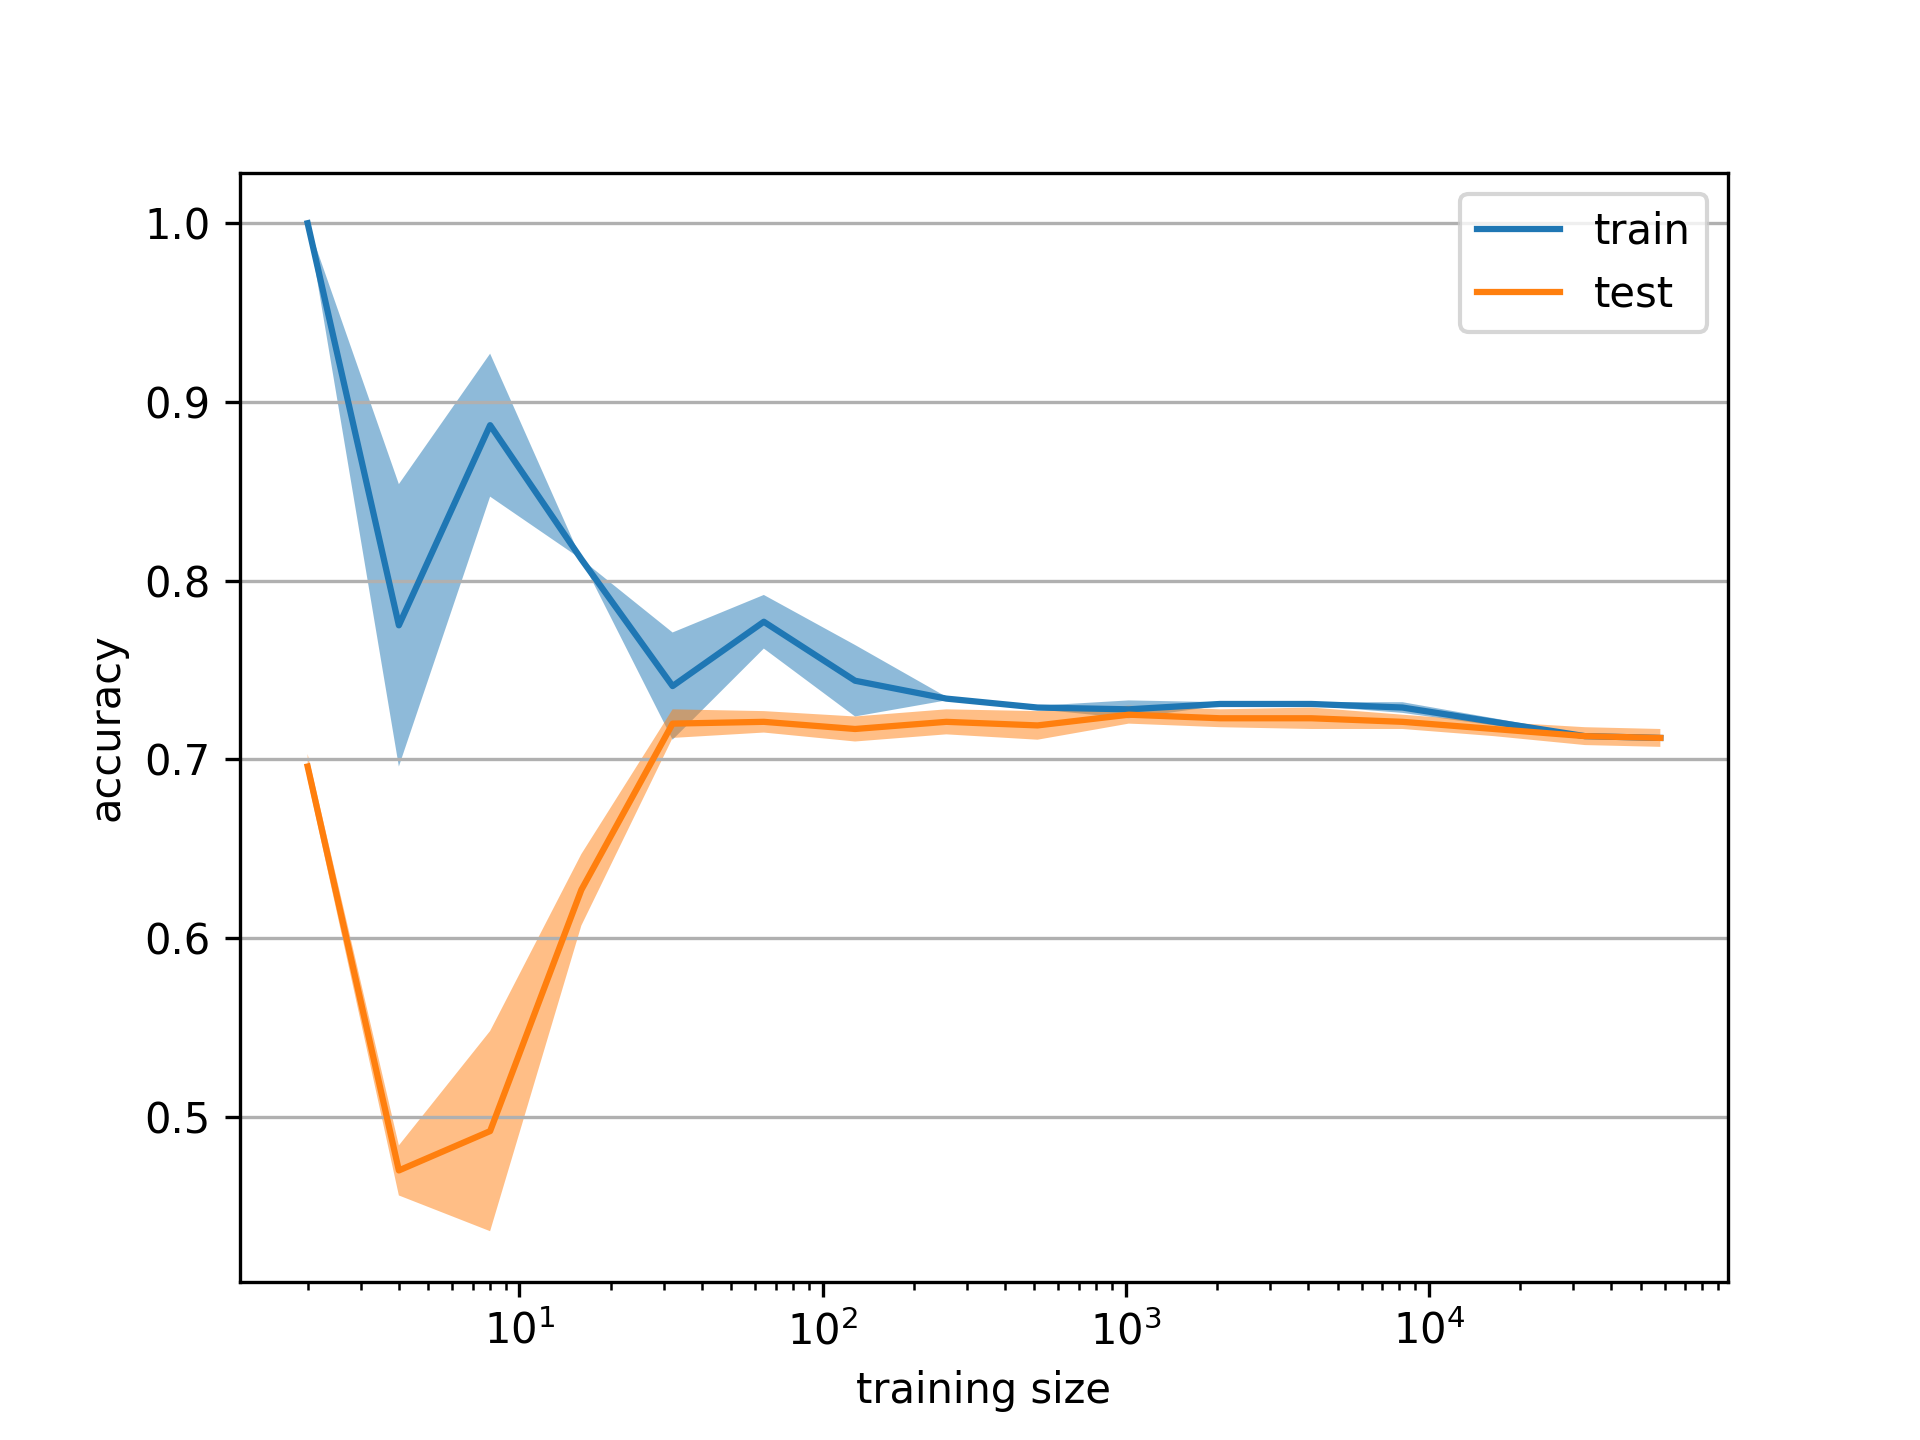
\includegraphics[width=130mm]{figures/lc2_acc.png}
\caption{Learning curves with standard deviation for Na\"{\i}ve Bayes --- accuracy}\label{fig:l_curves2_accuracy}
The x axis is log scaled.
\end{figure}

\begin{figure}[h]\centering
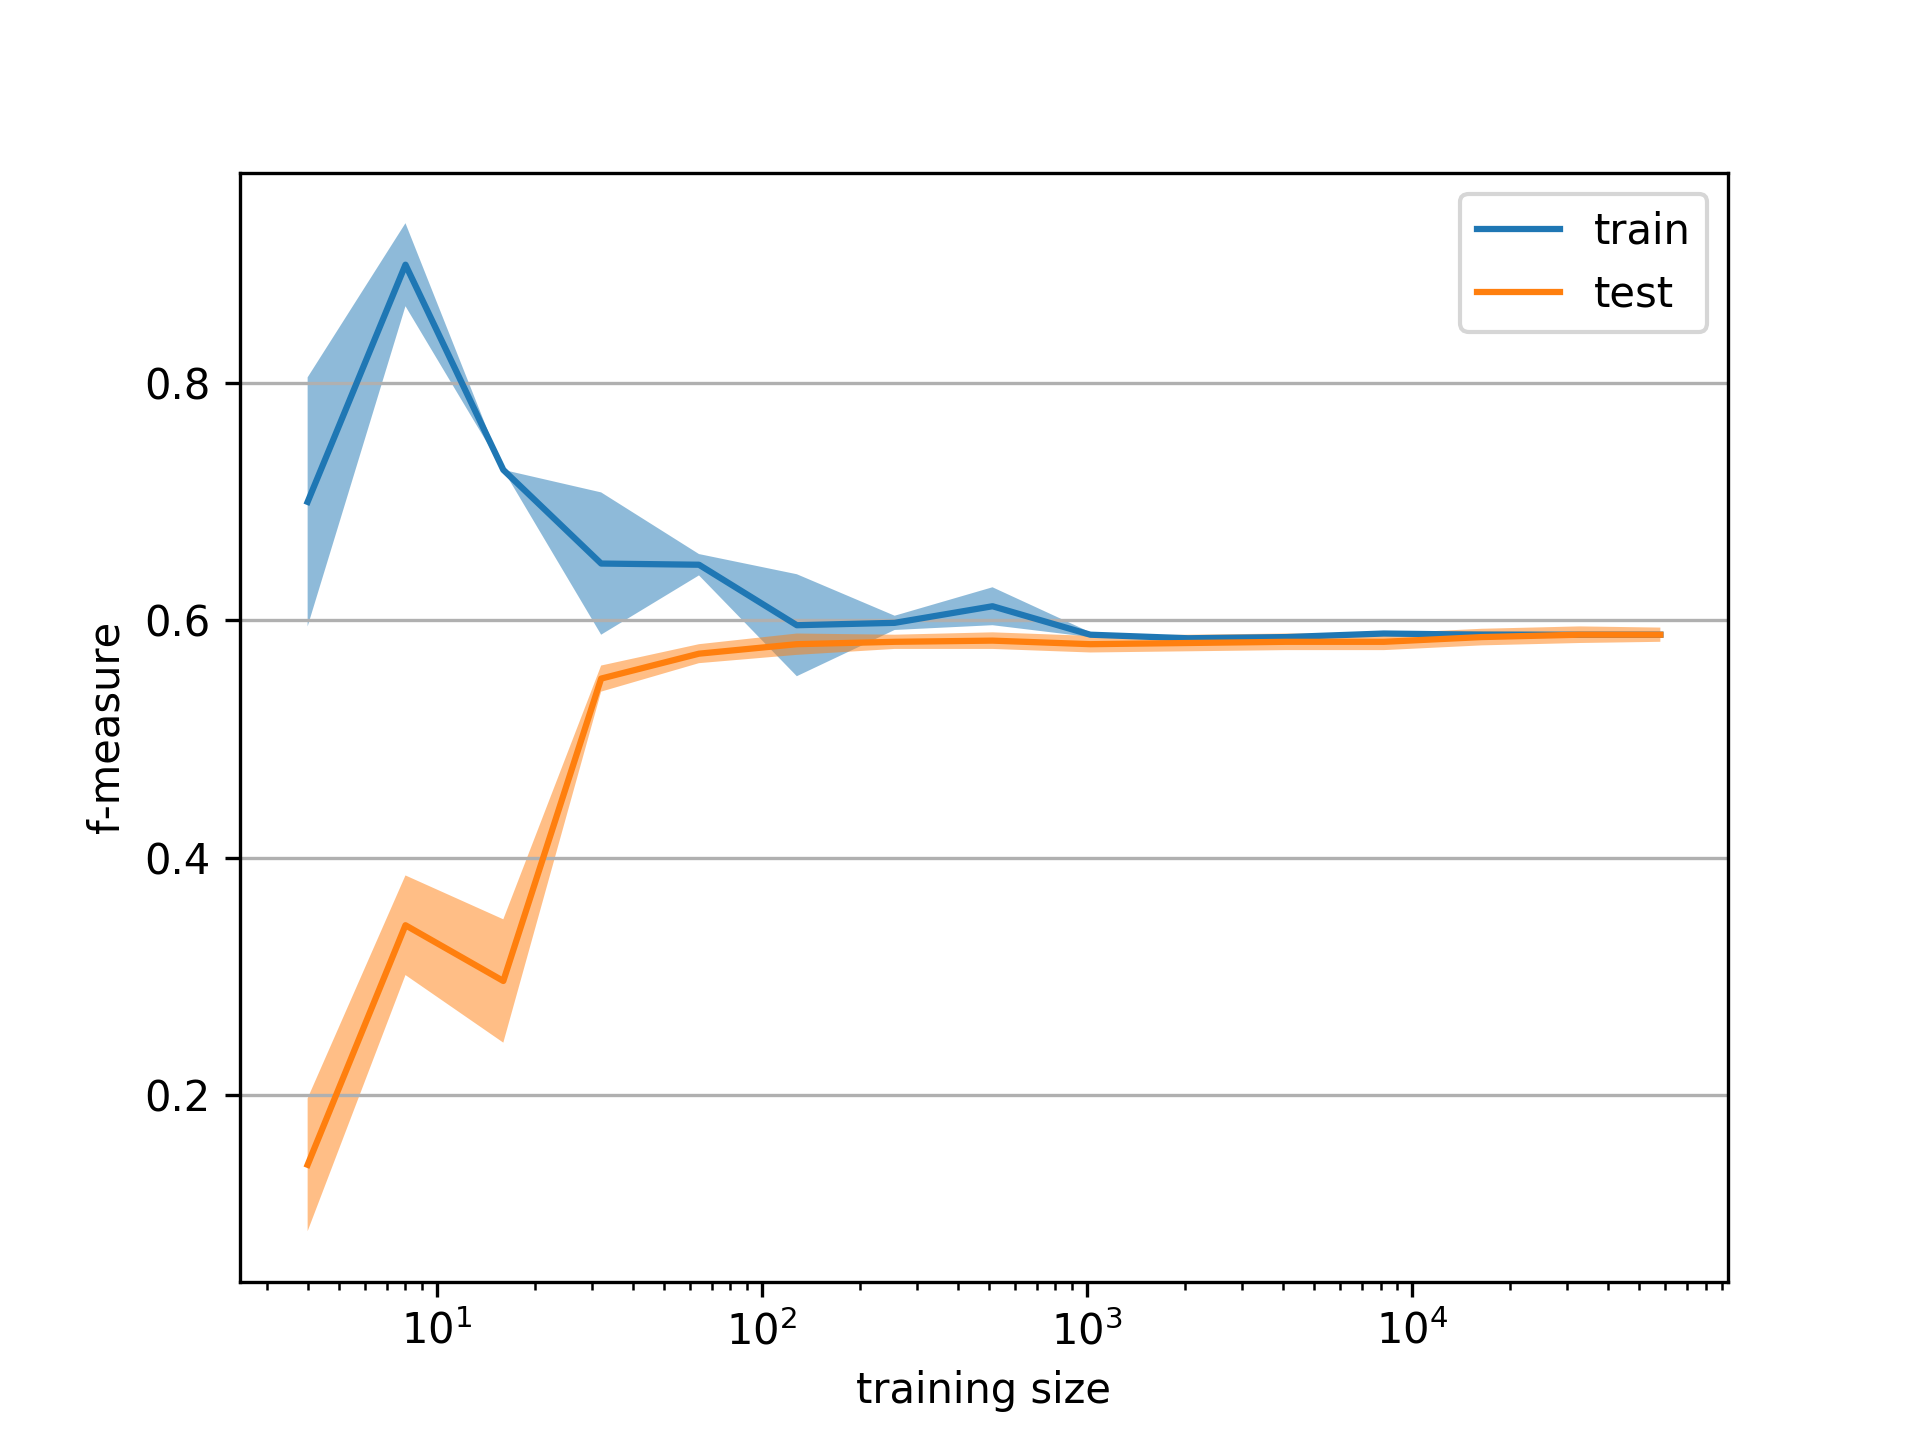
\includegraphics[width=130mm]{figures/lc2_fm.png}
\caption{Learning curves with standard deviation for Na\"{\i}ve Bayes --- f-measure}\label{fig:l_curves2_f_measure}
The x axis is log scaled.
\end{figure}


\begin{figure}[h]\centering
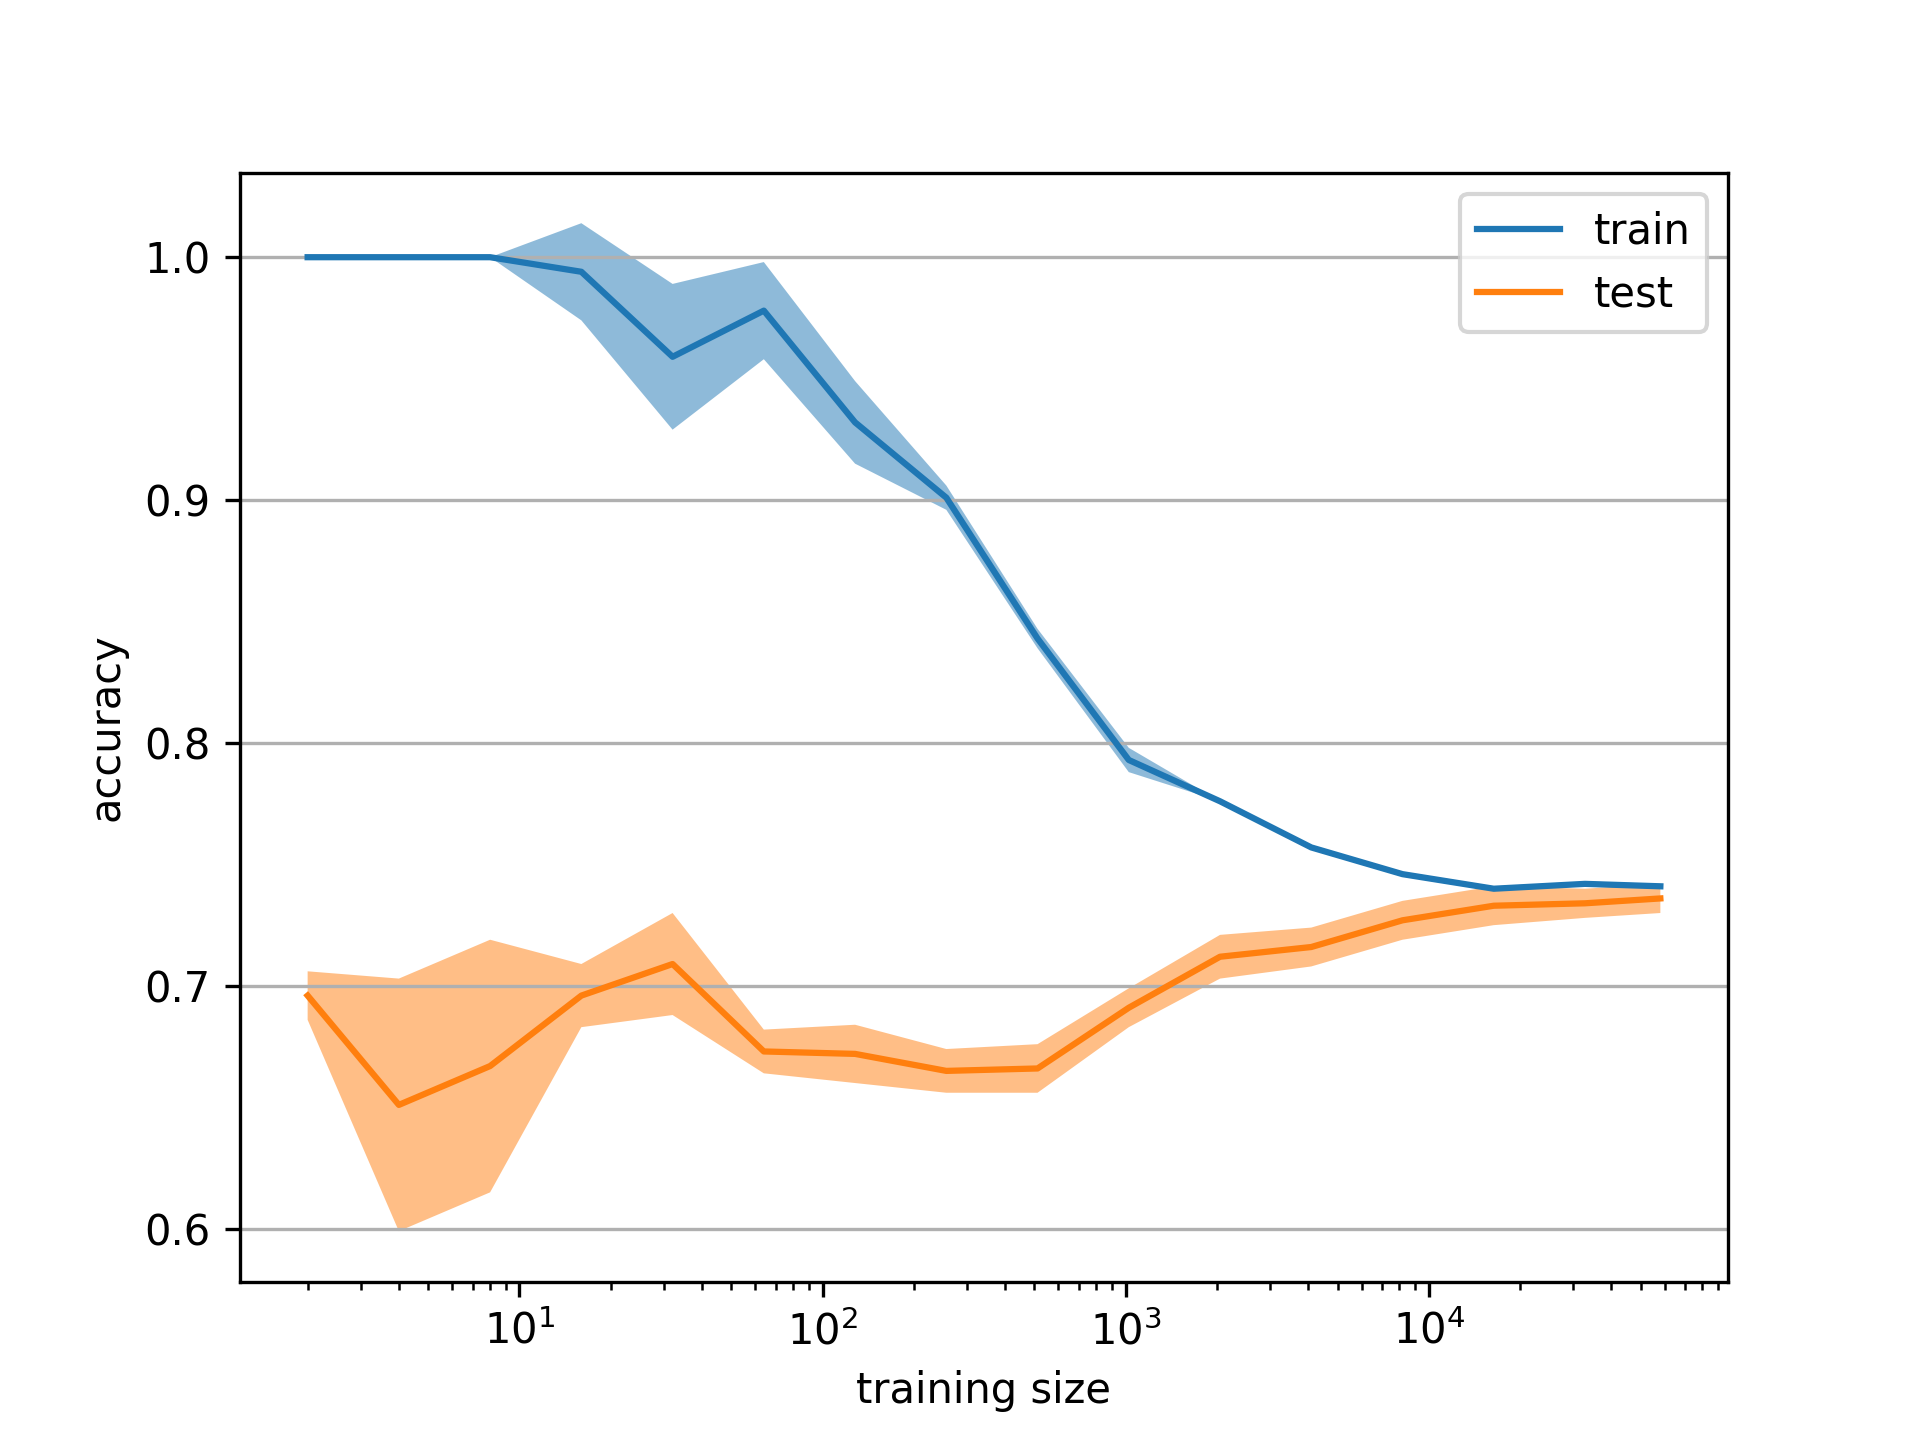
\includegraphics[width=130mm]{figures/lc3_acc.png}
\caption{Learning curves with standard deviation for decision tree --- accuracy}\label{fig:l_curves3_accuracy}
The x axis is log scaled.
\end{figure}

\begin{figure}[h]\centering
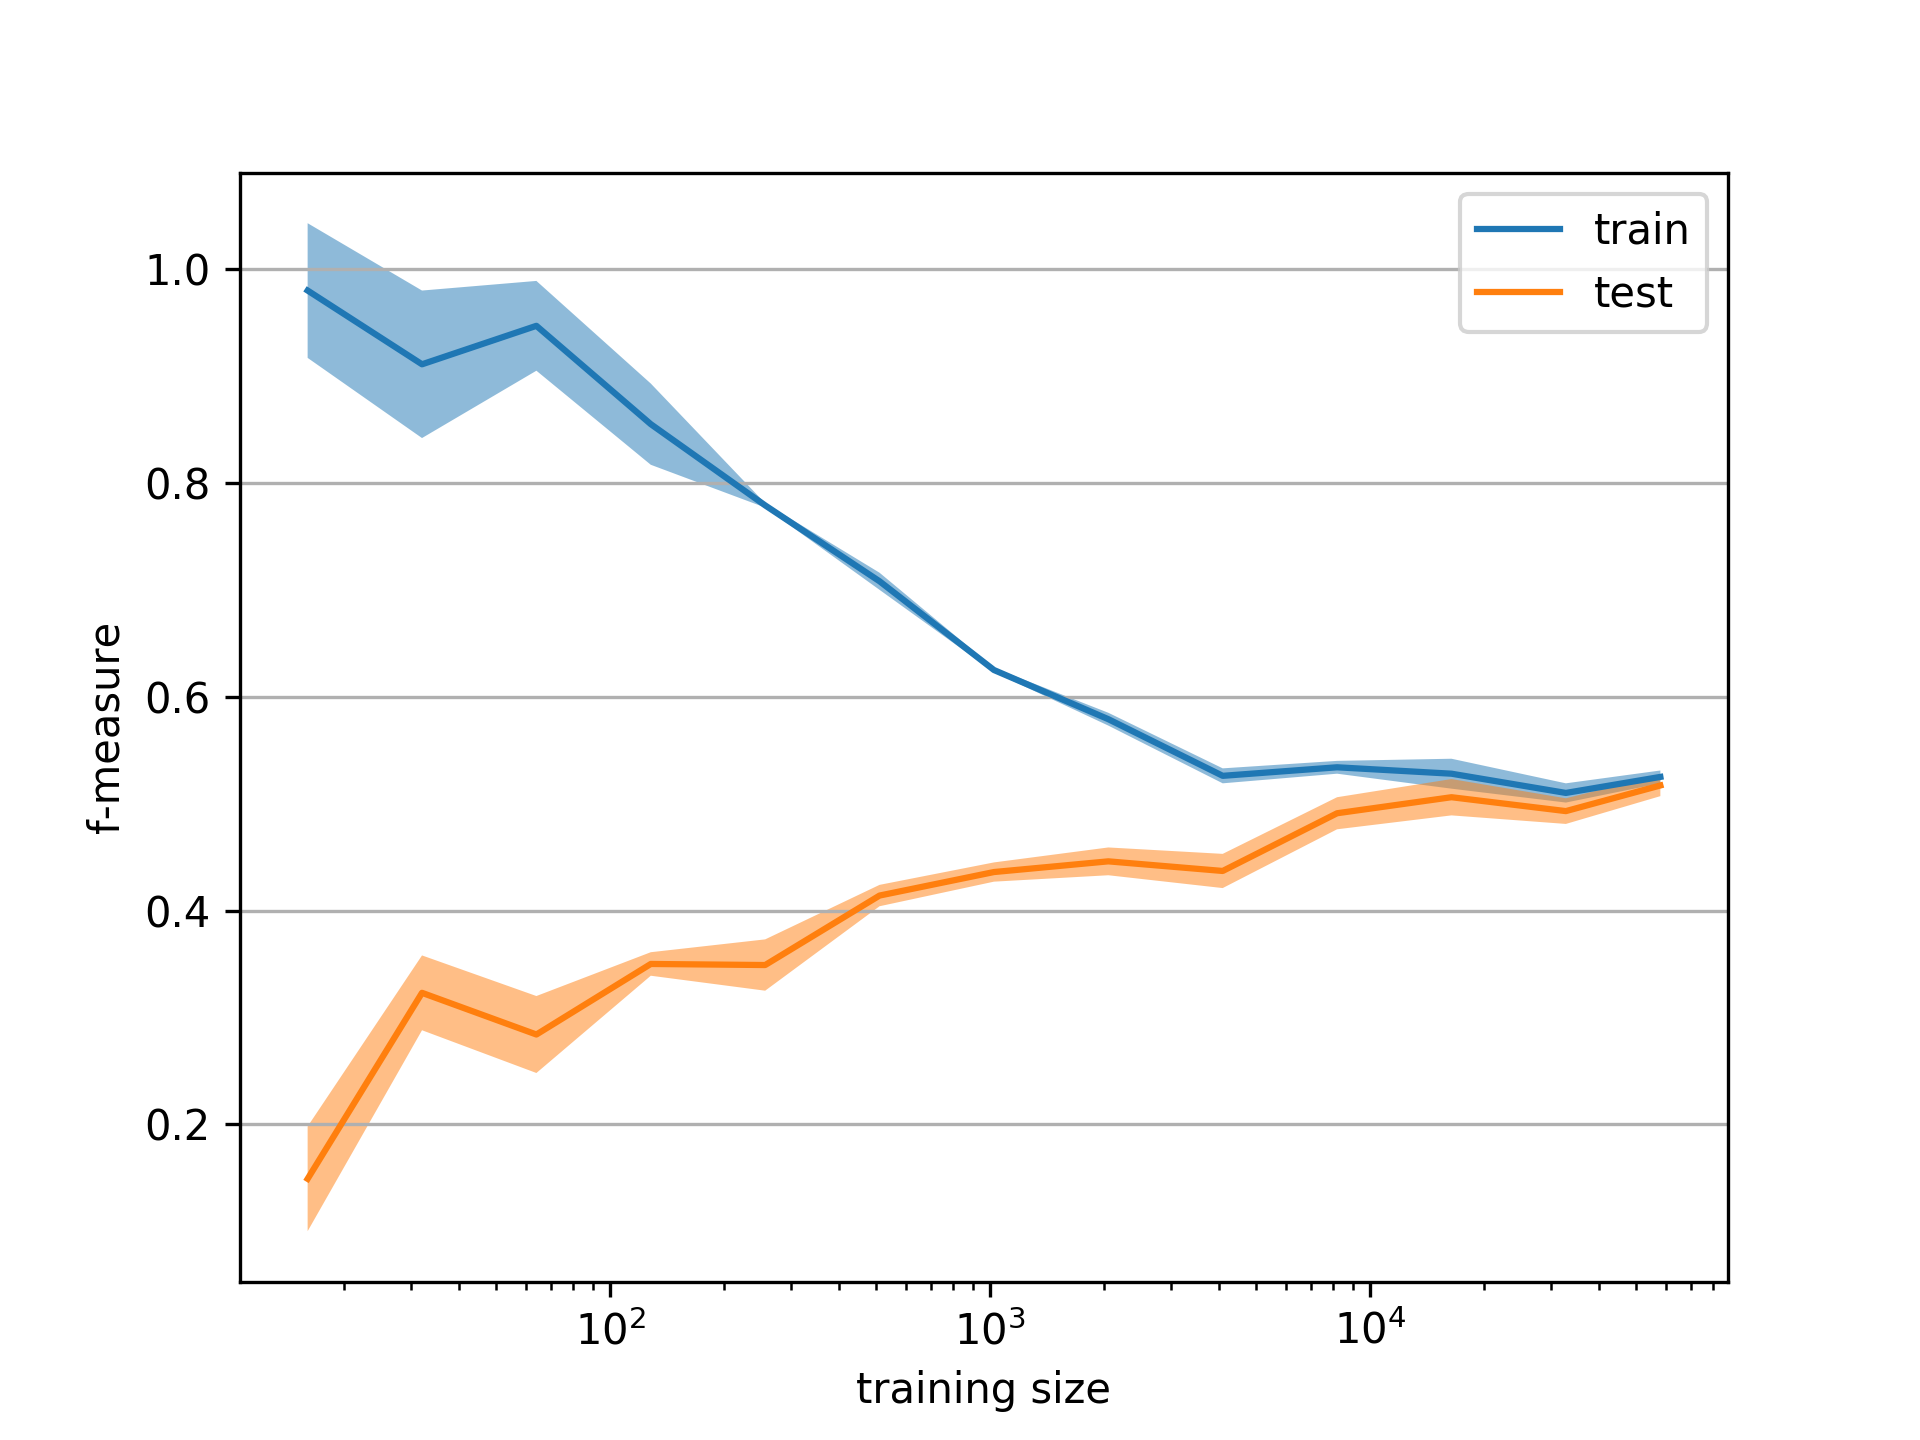
\includegraphics[width=130mm]{figures/lc3_fm.png}
\caption{Learning curves with standard deviation for decision tree --- f-measure}\label{fig:l_curves3_f_measure}
The x axis is log scaled.
\end{figure}


\chapter*{Conclusion}
\label{chap:concl}

\addcontentsline{toc}{chapter}{Conclusion}


\appendix
\addappheadtotoc
\appendix
\addappheadtotoc
%\addcontentsline{toc}{chapter}{Appendices}
\chapter{Yelp Dataset}\label{app:dataset}

Yelp is a US-based company whose goal is: ``to connect people with great local businesses.''\footnote{\url{https://yelp.com/about}}
It provides both mobile and web interface listing businesses such as restaurants or shopping centres.
Users can easily post a review for any business based on their recent visit.
Its convenience and usefulness makes the platform very popular.

It works in a similar manner like other recommnedation systems such as IMDB\footnote{Internet Movie Database \url{https://www.imdb.com/}} or
TripAdvisor.\footnote{\url{https://www.tripadvisor.com}}
There are restaurant profiles to which users can add reviews.
Users can search for restaurants based on various parameters as shown in \autoref{fig:filters}.

\begin{figure}[ht]\centering
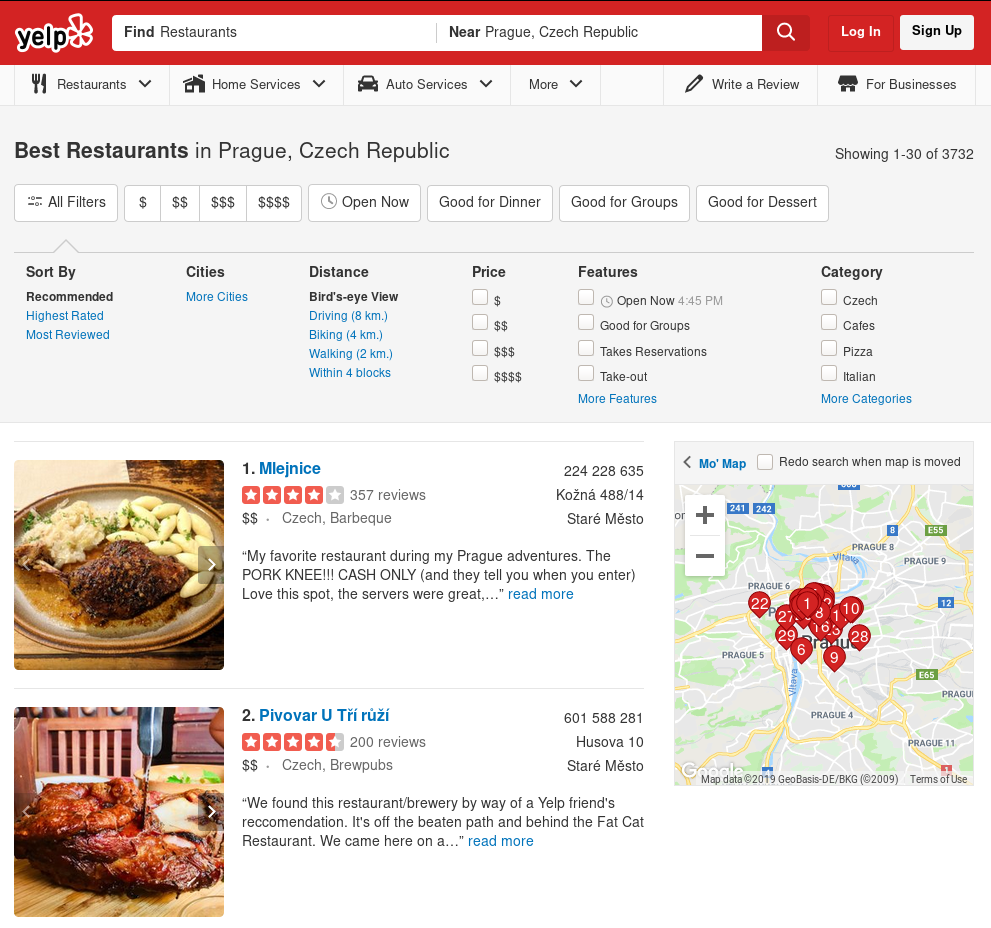
\includegraphics[width=130mm]{../img/filters.png}
\caption{Seeking restaurants with parameters}
\label{fig:filters}
\end{figure}

An example of a profile is shown in \autoref{fig:dobra_trafika}.
On the sides, various information such as price range or opening time is shown.
The main part is devoted to reviews.
Every review clearly displays the number of stars awarded and the text.
Also, Yelp already works with some sort of usefulness,
because two reviews have been hidden as can be seen in the bottom of the picture.

Yelp also allows users to flag properties of other reviews in the form of \emph{likes}.
Each review has three buttons --- \emph{useful}, \emph{funny} and \emph{cool} as can be seen in \autoref{fig:dobra_trafika}.
A user can vote for the property of a review by clicking on one of these buttons.

\begin{figure}[ht]\centering
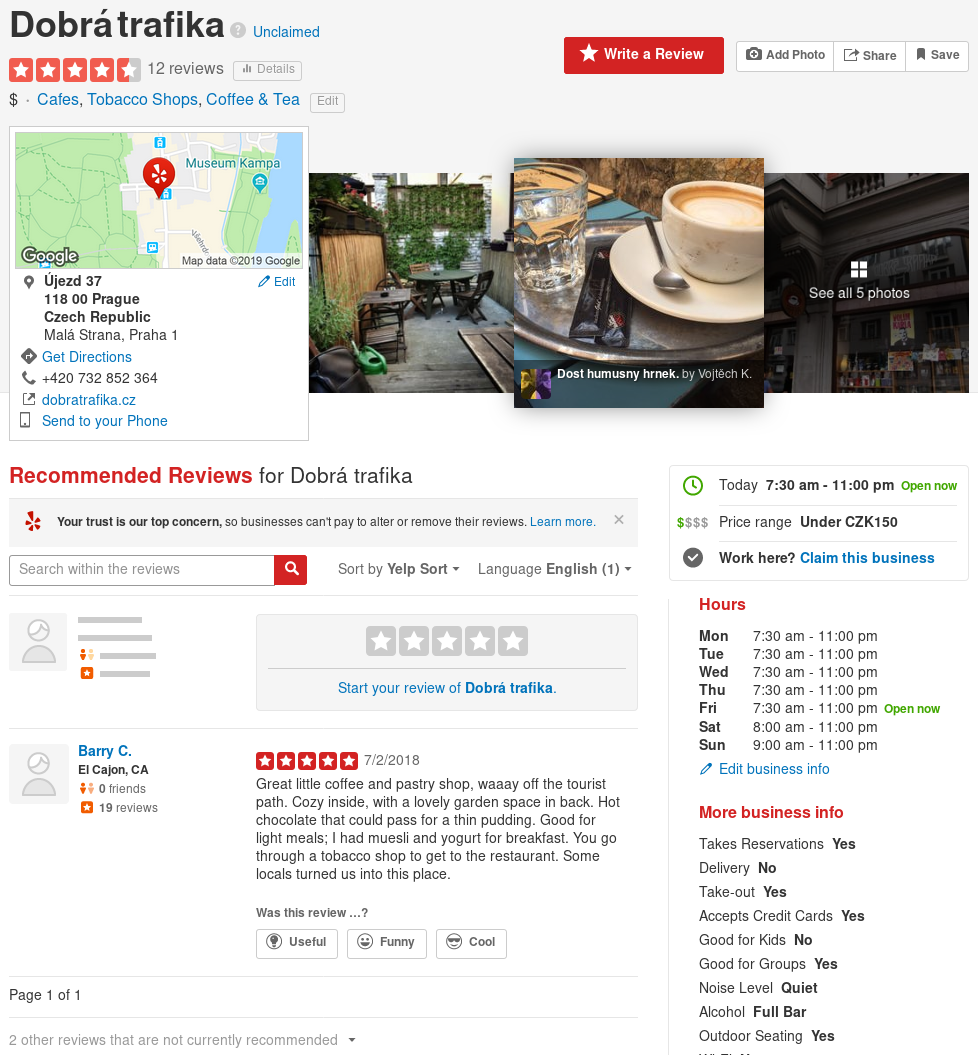
\includegraphics[width=130mm]{../img/dobra_trafika.png}
\caption{An example of an online profile}
\label{fig:dobra_trafika}
\end{figure}

There are three main reasons we chose Yelp reviews.

First, this platform is very popular and as such has sufficient data.

Secondly, the company publishes every year an open dataset which can be downloaded for academic
purposes.
It covers most information conveyed in their system ---  information about businesses and users, pictures taken by the users and textual reviews.
The data is available for download and we can focus on building our programme, rather than obtaining data.

Lastly, the dataset contains the information how many times the like buttons have been clicked on.
This allows us to asses the needed properties of individual reviews and
we use it to distinguish useful and not-useful reviews.

\section{Format of the Dataset}
\label{sec:format}

The Yelp Dataset contains various files.
We use files \texttt{review.json} and \texttt{business.json}.
The former contains reviews represented by JSON.
There is one review per line.\footnote{In fact, it is JSON lines format --- \url{https://jsonlines.org}}

Every review contains unique ID and business ID which is a reference to a business in file \texttt{business.json}.
It also contains data about the review itself; review text, date of publishing and number of individual likes it received so far.
Also, every review is acompanied by a star rating.
The interval is one to five stars; five being the best.
An example of a pretified review is bellow.

\begin{code}
{
	"review_id": "---nya_pjxWmNFDFyAcfsA",
	"user_id": "5QOtcHU1SoqEqBCRR6FhsA",
	"business_id": "zQNJwaWR1M1zDjLNVJiNEw",
	"stars": 1,
	"date": "2012-06-27",
	"text": "Another case of the Emperor's New Clothes...",
	"useful": 10,
	"funny": 2,
	"cool": 3
}
\end{code}

The second file we use is \texttt{business.json}.
Again, it is in JSON lines and it contains business information such as openning hours or availability of a car park.
An example of a business can be found bellow.

\begin{code}
{
	"business_id": "zQNJwaWR1M1zDjLNVJiNEw",
	"name": "Pizza M",
	"neighborhood": "",
	"address": "208 W Main St",
	"city": "Urbana",
	"state": "IL",
	"postal_code": "61801",
	"latitude": 40.112655,
	"longitude": -88.2093142,
	"stars": 3.5,
	"review_count": 60,
	"is_open": 1,
	"attributes": {
		"RestaurantsTableService": false,
		"Alcohol": "beer_and_wine",
		"Caters": false,
		"HasTV": false,
		"RestaurantsGoodForGroups": true,
		"NoiseLevel": "average",
		"WiFi": "free",
		"RestaurantsAttire": "casual",
		"RestaurantsReservations": false,
		"OutdoorSeating": false,
		"BusinessAcceptsCreditCards": true,
		"RestaurantsPriceRange2": 2,
		"BikeParking": true,
		"RestaurantsDelivery": true,
		"RestaurantsTakeOut": true,
		"GoodForKids": true,
		"BusinessParking": {
			"garage": true,
			"street": true,
			"validated": false,
			"lot": false,
			"valet": false
		}
	},
	"categories": ["Restaurants", "Pizza"],
	"hours": {
		"Monday": "11:00-21:00",
		"Tuesday": "11:00-21:00",
		"Friday": "11:00-22:00",
		"Wednesday": "11:00-22:00",
		"Thursday": "11:00-22:00",
		"Sunday": "11:00-21:00",
		"Saturday": "11:00-23:00"
	}
}
\end{code}

There are other files that could contain potentially useful information.
The file \texttt{user.json} is possibly interesting, because it contains information about users.
There is a cross reference from reviews to users in the same manner as businesses,
so we could get potentially useful information for every review;
for exampe the number of reviews already posted by the author or
how long the poster has been registred on Yelp.

We decided not to use this file for three main reasons.
First, the data is very sparse and it would be hard to avoid overfitting or gain significant improvement.
There is a lot of information about users resulting in very big denormalized data
and as such hard to work with.
Lastly and most importantly, this thesis focuses on extracting information from text rather than from metadata.
For this reason we also used business information only for filtering reviews,
but not for the actual classification.


\chapter{Data Preprocessing}\label{app:prepr}

One of the biggest problems with short text and online platforms in general is
the fluctuating quality.
In this chapter, we discuss how to filter reviews to get more reliable data with
less noise.
Next, we describe how we prepared the data to be directly fed into the classifiers.


\section{Filtering Reviews}

The number of likes is a problematic metric for usefulness.
Different reviews having the same ``level'' of usefulness can vary greatly
in the number of likes.
One of the biggest influences is the age of reviews and online popularity.
Also, the social group visiting the business has a considerable impact.
Locals going to the same pub for years will not produce nearly as much traffic
as a touristic spot.
Reviews for a club for young people will have different rates of visits and likes
than a place for families.

Using all reviews directly would therefore be problematic.
We tried to reduce the variance by filtering out reviews.
We use only reviews belonging to businesses with at least 50 reviews and 10 attributes.
This is to omit infrequently visited restaurants where the number of likes could fluctuate a lot.
Also, it avoids restaurants with incomplete online profile which may be less likely to be reviewed.
Lastly, we dropped all reviews with one and only one like.
One like may be a missclick or some other noise.

To avoid the problem with age, we used only reviews posted in a very specific date frame
--- between 1$^{st}$ May 2012 and 1$^{st}$ December 2012.
Thanks to this all reviews have been exposed for the same time to receive any likes.

Note that the dataset contains general businesses, but we focus on restaurants only.
When we analysed filtered reviews,
there were less than 30,000 reviews for non-restaurants out of total 206,000.
Because the rate is rather small,
we decided to treat all businesses the same way as restaurants.

Next, we needed to remove reviews in other language, because
we focus on English text only.
Besides English, two other languages (German and French) are frequently present.
We decided to filter out the two languages.
Other languages have been left intact, because they presence is not significant.

For language recognition, we used very simple approach.
We used the ratio of incorrect words to detect language.
We computed the ratio of misspelled and correct words for English, German and French and
picked the language with the lowest ratio.
It worked surprisingly well, even though many English words such as ``credit card'' or ``hamburger'' are used in the other languages too.

\section{Data Preparation}

For easier manipulation, we denormalized the data.
Also, we ran a spellchecker\footnote{\url{https://aspell.net}} on every review and added the information of number of words and number of misspelled words to the review.
We used the rate of misspelled words as a feature.

The resulting data has been saved in an instance file,
which is in JSON lines containing an instance per line.
An instance is a review with the element \texttt{business\_id} replaced by the business information.
An example of a full instance is bellow.

\begin{code}
{
	"review_id": "---nya_pjxWmNFDFyAcfsA",
	"user_id": "5QOtcHU1SoqEqBCRR6FhsA",
	"business_id": {
		"business_id": "zQNJwaWR1M1zDjLNVJiNEw",
		"name": "Pizza M",
		"neighborhood": "",
		"address": "208 W Main St",
		"city": "Urbana",
		"state": "IL",
		"postal_code": "61801",
		"latitude": 40.112655,
		"longitude": -88.2093142,
		"stars": 3.5,
		"review_count": 60,
		"is_open": 1,
		"attributes": {
			"RestaurantsTableService": false,
			"Alcohol": "beer_and_wine",
			"Caters": false,
			"HasTV": false,
			"RestaurantsGoodForGroups": true,
			"NoiseLevel": "average",
			"WiFi": "free",
			"RestaurantsAttire": "casual",
			"RestaurantsReservations": false,
			"OutdoorSeating": false,
			"BusinessAcceptsCreditCards": true,
			"RestaurantsPriceRange2": 2,
			"BikeParking": true,
			"RestaurantsDelivery": true,
			"RestaurantsTakeOut": true,
			"GoodForKids": true,
			"BusinessParking": {
				"garage": true,
				"street": true,
				"validated": false,
				"lot": false,
				"valet": false
			}
		},
		"categories": ["Restaurants", "Pizza"],
		"hours": {
			"Monday": "11:00-21:00",
			"Tuesday": "11:00-21:00",
			"Friday": "11:00-22:00",
			"Wednesday": "11:00-22:00",
			"Thursday": "11:00-22:00",
			"Sunday": "11:00-21:00",
			"Saturday": "11:00-23:00"
		}
	},
	"stars": 1,
	"date": "2012-06-27",
	"text": "Another case of the Emperor's New Clothes...",
	"useful": 10,
	"funny": 2,
	"cool": 3,
	"words": 57,
	"incorrect_words": 0
}
\end{code}



\chapter{Geneea Data}\label{app:geneea}

Geneea Analytics\footnote{\url{https://www.geneea.com}} is a company focusing on natural language processing.
We used their analysing tools extract additional linguistics properties.

The reviews were analysed and filtered on Geneea servers.
The resulting file is transferred to the local computer.
It has line-by-line correspondence to the instance file created locally.
An example of an analyzed review is bellow.
Note that we omitted unused parts of analysis; full analysis can be found in \texttt{data/geneea\_sample.json}.

\begin{code}
{
  "text": "Another case of the Emperor's New Clothes...",
  "language": {
    "value": "en"
  },
  "sentiment": {
    "value": -0.04392095867614757,
    "label": "neutral",
    "sentenceVals": [
      0.0,
      0.373666763147296,
      -0.27144176165949063,
      -0.32182979486854324,
      0.0
    ]
  },
  "entities": [
    {
      "standardForm": "limited hour",
      "type": "phrase",
      "links": {},
      "instances": [
        {
          "text": "NSUBJ:hours(AMOD:limited)",
          "mwLemma": [
            "limited",
            "hour"
          ],
          "sentiment": -0.010824959347792613,
          "tokenIndices": [
            43,
            44
          ],
          "segment": "text",
          "offset": 226
        }
      ]
    },
    {
      "standardForm": "good fare",
      "type": "phrase",
      "links": {},
      "instances": [
        {
          "text": "NSUBJ:fare(AMOD:good)",
          "mwLemma": [
            "good",
            "fare"
          ],
          "sentiment": 3.6455297098939717e-09,
          "tokenIndices": [
            18,
            21
          ],
          "segment": "text",
          "offset": 97
        }
      ]
    },
	...
  ],
  "id_idx": "4362382",
  "id": "---nya_pjxWmNFDFyAcfsA"
}

\end{code}

This analysis is loaded with the geneea public SDK\footnote{\url{https://help.geneea.com/sdk/index.html}}.
We use entities and sentiment.

\chapter{Package Technicalities}\label{app:techn}

The entire project runs in Python of version at least 3.6\footnote{\url{https://python.org}} and bash\footnote{\url{https://gnu.org/software/bash}}.
The following libraries are used:

\begin{table}[h]
\centering
\begin{tabular}{ll}
\toprule
\textbf{library} & \textbf{purpose} \\
\midrule

nltk & tokenizer, Na\"{i}ve Bayes\\
pandas & DatFrame for storing raw data in memory\\
scipy & sparse matrix for storing features\\
yaml & parser for configuration file \\
geneea-nlp-client & parser for loading Geneea analysis\\
gensim & compute cosine similarity \todoA{unused} \\
fasttext & classification model \\
aspell & spell checking \\


\bottomrule
\end{tabular}

\caption{Used libraries}\label{tab:libs}
\end{table}

The project is executed with make\footnote{url{https://www.gnu.org/software/make}}.
The entire project can be run by:

\begin{code}
make run
\end{code}

Or for demonstration running with a small subset of data:

\begin{code}
make run_sample
\end{code}

Because Geneea analysis is carried out remotely, \texttt{make} will prompt user for copying that file when appropriate.

Results are stored in \texttt{graphs/\textit{timestamp}}.
A new folder for statistics is created every run to prevent accidental overwriting of already obtained results.


\section{Experiments File}

This YAML\footnote{\url{https://yaml.org}}  file contains entire configuration of experiments conducted.
It lists classification tasks and specifies graphs to be plotted.
Each task is a definition of a classifier.
Evaluation element is a definition what properties should be plotted in a graph.

Experiments file has the following format.
The root element is a dictionary with three parts;
\texttt{config}, \texttt{tasks} and \texttt{graphs}.
An example file can be found bellow.

\begin{code}
config:
  chunks: 10
  mi: true
  l_curves: false
  max_ngrams: 100
  max_tfidf: 100
tasks:
  - name: 'zero-R'
    classificator: 'baseline'
    features:
      - REVIEWLEN
      - UNIGRAMS
    preprocessing:
      - 'mutualinformation'
      - 'featurematrixconversion'
    extra_data: []
    config:
      algorithm: 'zero-R'
      features_to_select: 2
graphs:
  - name: 'baseline'
    data:
      zero-R:
        - 'f-measure'
\end{code}

The config section is a dictionary.
It must contain the elements specified in \autoref{tab:config_yaml}.

\begin{table}[h]
\centering
\begin{tabular}{lll}
\toprule
\textbf{key} & \textbf{datatype} & \textbf{value} \\
\midrule

chunks & int & parameter $k$  k-fold crossvalidation\\
mi & bool & if mutual information should be calculated\\
l\_curves & bool & ordinary/learning curves evaluation\\
max\_ngrams & int & number of unigrams used \\
max\_tfidf & int & number of words for TF-IDF used\\

\bottomrule
\end{tabular}

\caption{Config section}\label{tab:config_yaml}
\end{table}


The section \texttt{experiments} is a list of classification tasks.
Each element is a dictionary specifying the exact parameters.
Descriptions of individual fields is in \autoref{tab:exp_dict}.
The list \texttt{features} consists of names as defined in FeatureSetEnum.
The exact definition can be found in \autoref{tab:fea_grp}.
\texttt{extra\_data} is any property of instances available in the raw data.
An example is the original text or business attributes.

\begin{table}[h]

\centering
\begin{tabular}{lll}
\toprule
\textbf{element name} & \textbf{type} & \textbf{meaning}\\
\midrule
name 			& string	& identification referred to in graphs\\
classificator 	& string	& used classifier\\
features 		& list		& used features \\
preprocessing 	& list		& applied preprocessors in order\\
extra\_data 	& list 		& extra attributes passed to the first preprocessor \\
config			& dict		& extra configuration for all parts of pipeline \\
\bottomrule
\end{tabular}

\caption{Experiment Configuration}\label{tab:exp_dict}
\end{table}


The last section \texttt{graphs} is used for specifying what graphs will be plotted.
It is a list of individual figures.
Each figure is a dictionary of two elements; \texttt{name} and \texttt{data}.
Name specifies the filenames of the resulting graph ---
for each figure png and csv files will be created.
Element \texttt{data} specifies what evaluation metrics for what classifiers will be used.
It is a dictionary of experiment names, values being a list of all metrics to be output.





TADY KONEc

\autoref{tab:files} displays definitions of special files used for controlling the run of the software project.
Their exact usage is explained in appropriate sections.

The preprocessors are in the same order as in the experiment file.
A preprocessor must be defined in the directory \texttt{preprocessors} and be a child of \texttt{preprocessors/preprocessingbase.py}.
Also, its name must be added into \texttt{preprocessors/\_\_init\_\_.py}.

Since the input and output formats of the pipeline units are arbitrary,
it is up to the user to ensure compatibility of adjacent units.
This holds except for the input of the first preprocessor and the output of the classifier.
The first preprocessor in the pipeline must take feature\_dict with possibly additional data specified in \texttt{extra\_data} as returned by \texttt{load\_data.Data.get\_feature\_dict}.
The classifier must return the predicted label.
The output of training is not stored.
Note that for most classifiers, it is needed to run conversion to matrix as a last preprocessor (\texttt{featurematrixconversion.py}).

and classifier is called train and classify for
training and testing data, respectively.
The pipeline is the same for both training and testing data with the guarantee that
training data is always passed first.


%%% Bibliography
%%% Bibliography (literature used as a source)
%%%
%%% We employ bibTeX to construct the bibliography. It processes
%%% citations in the text (e.g., the \cite{...} macro) and looks up
%%% relevant entries in the bibliography.bib file.
%%%
%%% The \bibliographystyle command selects, which style will be used
%%% for references from the text. The argument in curly brackets is
%%% the name of the corresponding style file (*.bst). Both styles
%%% mentioned in this template are included in LaTeX distributions.

\bibliographystyle{plainnat}    %% Author (year)
% \bibliographystyle{unsrt}     %% [number]

\renewcommand{\bibname}{Bibliography}

%%% Generate the bibliography. Beware that if you cited no works,
%%% the empty list will be omitted completely.

\bibliography{bibliography}

%%% If case you prefer to write the bibliography manually (without bibTeX),
%%% you can use the following. Please follow the ISO 690 standard and
%%% citation conventions of your field of research.

% \begin{thebibliography}{99}
%
% \bibitem{lamport94}
%   {\sc Lamport,} Leslie.
%   \emph{\LaTeX: A Document Preparation System}.
%   2nd edition.
%   Massachusetts: Addison Wesley, 1994.
%   ISBN 0-201-52983-1.
%
% \end{thebibliography}


%%% Figures used in the thesis (consider if this is needed)
\listoffigures

%%% Tables used in the thesis (consider if this is needed)
%%% In mathematical theses, it could be better to move the list of tables to the beginning of the thesis.
\listoftables
\XXX{In mathematical theses, it could be better to move the list of tables to the beginning of the thesis.}

%%% Abbreviations used in the thesis, if any, including their explanation
%%% In mathematical theses, it could be better to move the list of abbreviations to the beginning of the thesis.
\chapwithtoc{List of Abbreviations}
\XXX{In mathematical theses, it could be better to move the list of abbreviations to the beginning of the thesis.}

%% PHDONLY
%%% Doctoral theses must contain a list of author's publications
\chapwithtoc{List of publications}
\XXX{Doctoral theses must contain a list of author's publications.}
%% ONLYPHD

%%% Attachments to the bachelor thesis, if any. Each attachment must be
%%% referred to at least once from the text of the thesis. Attachments
%%% are numbered.
%%%
%%% The printed version should preferably contain attachments, which can be
%%% read (additional tables and charts, supplementary text, examples of
%%% program output, etc.). The electronic version is more suited for attachments
%%% which will likely be used in an electronic form rather than read (program
%%% source code, data files, interactive charts, etc.). Electronic attachments
%%% should be uploaded to SIS and optionally also included in the thesis on a~CD/DVD.
%%% Allowed file formats are specified in provision of the rector no. 72/2017.
\appendix
\chapter{Attachments}
\XXX{Attachments to the bachelor thesis, if any. Each attachment must be referred to at least once from the text of the thesis. Attachments are numbered.}
\XXX{The printed version should preferably contain attachments, which can be read (additional tables and charts, supplementary text, examples of program output, etc.). The electronic version is more suited for attachments which will likely be used in an electronic form rather than read (program source code, data files, interactive charts, etc.). Electronic attachments should be uploaded to SIS and optionally also included in the thesis on a~CD/DVD. Allowed file formats are specified in provision of the rector no. 72/2017.}

\section{First Attachment}

\openright
\end{document}
